\documentclass{osr}
\usepackage{stfloats}
\usepackage{wrapfig}
\usepackage[frenchb]{babel}

\title{La tombe des rois serpents}
\author{}
\coverimage{pics/cover2.jpg}
%\covercolor{LimeGreen}
\covercolor{Emerald}
\abstract{\centering Un module "d'apprentissage" dans un style old school, conçu
  pour aider les nouveaux joueurs et les MJ à apprendre les éléments de base
  de l'exploration de donjons classiques et du pillage de tombes.}


\begin{document}

\maketitle
\thispagestyle{empty}

\tableofcontents

\chapter{Introduction}

La création de personnage pour Old School Essentials se fait traditionnellement de la manière suivante~:
\begin{enumerate}
  \item Tirez les caractéristiques
  \item Choisissez une classe
  \item Ajustez les caractéristiques
  \item Notez les modificateurs des caractéristiques
  \item Notez les valeurs d'attaque
  \item Notez scores de sauvegarde et capacités de classe
  \item Tirez vos points de vie
  \item Choisissez l'alignement
  \item Notez les langues connues
  \item Achetez votre équipement
  \item Notez votre Classe d'armure
  \item Notez votre niveau et vos XP
  \item Baptisez votre personnage
\end{enumerate}

Ce livret a pour objectif de remplacer les étapes 1 à 3 par une méthode inspîrée des playbooks du jeu \emph{Beyond the Wall and Other Adventures}\footnote{\url{https://www.flatlandgames.com/btw/}}.

Cette approche doit permettre
\begin{itemize}
  \item De fournir un historique basique au personnage
  \item D'assurer des valeurs caractéristiques qui correspondent à la classe choisie
\end{itemize}

\subsection{Création de personnages basée sur l'historique}
Appliquez successivement les étapes suivantes~:
\begin{enumerate}
  \item Déterminez la valeur initiale des caractéristiques~:
        Lancez 1D4+5 pour chacune d'entre elles.
  \item Déterminez les étapes importantes de votre enfance.
        Pour chacune des 3 tables du chapitre \nameref{chilhoud}~:
        \begin{itemize}
          \item Lancez le dé correspondant
          \item Notez l'élément d'historique obtenu
          \item Notez le bonus de caractéristique obtenu
        \end{itemize}
  \item Choisissez votre classe.
%        Les valeurs de caractéristiques que vous avez obtenu à l'étape précédente peuvent orienter votre choix.
  \item Déterminez les étapes importantes de votre formation.
        Référez vous au chapitre correspondant à votre classe (\nameref{warrior}, \nameref{mage}, \nameref{cleric}, \nameref{thief}, \nameref{dwarf}, \nameref{elf} ou \nameref{halfling}).
        Notez le bonus spécifique à chaque classe, puis,
        pour chacune des 4 tables de la formation~:
        \begin{itemize}
          \item Lancez le dé correspondant
          \item Notez l'élément d'historique obtenu
          \item Notez le bonus de caractéristique obtenu
        \end{itemize}
        \textbf{Note~:} Si la somme des bonus pour une caractéristique dépasse 18, ignorez le bonus ou retirez sur la table.
  \item Calculez vos valeurs de caractéristiques en ajoutant les bonus obtenus.
  \item Notez l'équipement obtenu
\end{enumerate}

\ifmulticolEnd
\section*{Notes de conception}
La méthode traditionnelle distribue toutes les caractériques de la même manière, sur une distribution en cloche centrée autour de la valeur 10,5.

La méthode proposée permet de favoriser selon la classe une caractéristique principale et deux secondaires.

\begin{osrtable}{XXXXXXXXX}{1}
Caractéristique  & Guerrier   & Mage     & Clerc    & Voleur   & Nain     & Elfe     & Halfelin & Moyenne \\
Principale       &  FOR       & INT      & SAG      & DEX      & CON      & INT      & DEX      & 13.15          \\
Secondaire       &  CON; DEX  & DEX; SAG & CON; CHA & INT; CHA & FOR; SAG & DEX; SAG & CON; SAG & 12.15          \\
Autres           &            &          &          &          &          &          &          & 10.15 \\
\end{osrtable}

\chapter{Niveau 1 : La Fausse Tombe}
\section{Structure}
Cette section introduit les bases de la conception et exploration de donjon en 7 salles.

Elle est pile de la bonne longueur pour une première session, pourvu que la création de personnages ait été rapide et que vous ayez donné aux PJ une bonne raison d'explorer la tombe.

Elle symbolise la joie de la découverte, le moment où l'on se dit \emph{"Oh ! Je vois !"} et l'anticipation du trésor à venir.

Assurez-vous de féliciter tout joueur parvenant à déduire qu'il s'agit d'une fausse tombe : l'astuce se doit d'être récompensée.

\newpage
\section{Description}
Décrivez cette zone avec des mots comme "branlant", "décrépi" et "humide".
C'est une vieille cave.
De petites racines blanches pendent du plafond pour venir lécher le sol.

\begin{center}[
  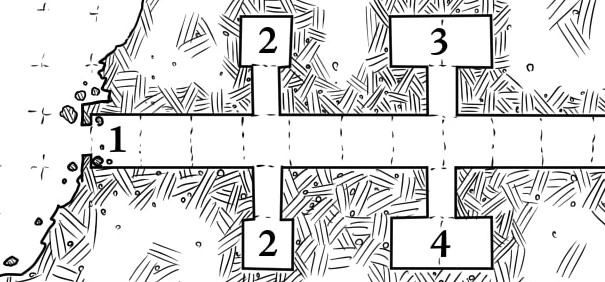
\includegraphics[width=\linewidth]{pics/map_1-4.jpg}
\end{center}

\subsection{1 : Hall d'Entrée}\label{n1:s1}
\begin{itemize}
  \item 37m de long, sur 3m de large et 3m de haut.
  \item La lumière du soleil en atteint l'extrémité.
  \item Sent la \textbf{poussière}. Plus \textbf{froid} qu'à l'extérieur.
  \item Fines racines au plafond, \textbf{roche taillée grossièrement}
  \item 2 ouvertures de 1.5m de large chaque côté.
  \item Se termine par une porte barrée menant en \textbf{\nameref{n1:s6}}.
\end{itemize}

\subsection{2 : Tombes des Gardes}\label{n1:s2}
\begin{itemize}
  \item Salle de 3m sur 3m, 2.5m de haut
  \item Sent la \textbf{poussière} et le \textbf{vieux bois}, avec un léger \textbf{relent acide}.
  \item Roche taillée grossièrement,
  \item Fresques de serpents entrelacés.
  \item Un \textbf{cercueil de bois} orné de gravures de scènes de bataille. Renferme :
  \begin{itemize}
    \item Statue de \emph{guerrier} en argile creuse, contient :
    \begin{itemize}
      \item une amulette d'or (10 PO)
      \item un squelette de serpent desséché
    \end{itemize}
    \item \textbf{Piège :} nuage de gaz empoisonné (Sauvegarde Poison ou 1d6 dégâts)
  \end{itemize}
\end{itemize}

\vfill*\columnbreak
\subsection{3 : Tombe d'Érudit}\label{n1:s3}
\begin{itemize}
  \item Salle de 6m sur 3m, 2.5m de haut
  \item Sent la \textbf{poussière} et le \textbf{tissu putréfié}
  \item Roche taillée grossièrement
  \item Fresques de serpents bondissants.
  \item Un \textbf{cercueil de bois} orné de gravures abstraites, renferme :
  \begin{itemize}
    \item Statue d'\emph{érudit} creuse
    \begin{itemize}
      \item une amulette d'or (10 PO)
      \item un squelette de serpent desséché
    \end{itemize}
    \item Parchemins tombés en poussière
    \item \textbf{Piège :} nuage de gaz empoisonné (Sauvegarde Poison ou 1d6 dégâts)
  \end{itemize}
\end{itemize}

\subsection{4 : Tombe de Sorcier}\label{n1:s4}
\begin{itemize}
  \item Salle de 6m sur 3m, 2.5m de haut
  \item Sent la \textbf{poussière} et le \textbf{tissu putréfié}
  \item Roche taillée grossièrement
  \item Fresques de serpents bondissants.
  \item Un \textbf{cercueil de bois} orné de gravures macabres, renferme :
  \begin{itemize}
    \item Statue de \emph{sorcier} creuse
    \begin{itemize}
      \item une amulette d'or (10 PO)
      \item un squelette de serpent desséché
    \end{itemize}
    \item \textbf{Piège :} nuage de gaz empoisonné (Sauvegarde Poison ou 1d6 dégâts)
    \item Porte un anneau d'argent. Si arraché :
    \begin{itemize}
      \item Brise la statue
      \item Projette le poison
    \end{itemize}
  \end{itemize}
\end{itemize}

\begin{highlight}[Anneau d'argent]
  \vspace*{-\baselineskip}
  \begin{itemize}
    \item magique \textbf{et} maudit
    \item Porté au doigt, l'ongle s'allonge et bifurque en deux pointes aiguisées comme des crocs.
    \item Mêmes effet qu'une dague empoisonnée :
    \item Chaque matin  : Sauvegarde contre le poison ou 1d6 dégâts.
    \item Si 6 dégâts :  le doigt tombe et se transforme en serpent.
  \end{itemize}
\end{highlight}

%\begin{highlight}
%\textbf{Leçons :} Les trésors cachés peuvent être magiques, utiles et parfois maudits.
%\end{highlight}

%\newpage
\subsection{5 : Porte / Marteau}\label{n1:s5}
Le corridor se termine par une \textbf{porte barrée}.
Deux pieux de fer plantés de chaque côté du chambranle soutiennent une lourde barre de pierre, bloquant l'accès à la salle suivante.

\begin{itemize}
  \item 3 PJ au moins pour la soulever
  \item \textbf{Soulevée :} Piège (Sauvegarde Mort ou 2d6+4 dégâts).
\end{itemize}

\begin{highlight}[Le piège]
  \vspace*{-\baselineskip}
  \begin{itemize}
    \item Marteau de pierre bascule du plafond
    \item Remplit \emph{presque} intégralement le couloir
    \item \textbf{\'Eviter :}
    \begin{itemize}
      \item Se plaquer au mur
      \item S'aider d'un autre PJ pour prendre appui : +2 au jet, -2 à l'autre PJ.
    \end{itemize}
    \item \textbf{Détection :}
    \begin{itemize}
      \item Examiner la porte, le plafond
      \item Examiner les pieux : se redressent lentement lorsque la barre est soulevée
    \end{itemize}
    \item \textbf{Désactiver :}
    \begin{itemize}
      \item Replacer la barre
      \item Maintenir les pieux en position basse
      \item Endommager le mécanisme au plafond
    \end{itemize}
  \end{itemize}
\end{highlight}

À moins que quelque chose ne le bloque, le marteau se rétracte lentement dans le plafond.

Il peut être activé à nouveau en abaissant les pieux de fer, à la main ou avec une corde.

L'impact force violemment l'ouverture des portes menant en \textbf{\nameref{n1:s6}}

\subsection{7 : Faux Temple}\label{n1:s7}
\begin{itemize}
  \item Salle de 6m sur 6m, 3m de haut
  \item Sent  fortement le \textbf{moisi},et la \textbf{pierre humide}
  \item \textbf{Statue d'un dieu homme-serpent}.
  \begin{itemize}
    \item Gigantesque, Hideux
  \end{itemize}
  \item Eau suinte du plafond
  \item L'eau a érodé le sol
  \item S'infiltre sous la statue :
  \begin{itemize}
    \item Révèle \textbf{\nameref{n2:s8}} vers le \textbf{\nameref{n2}} du donjon
  \end{itemize}
\end{itemize}
%\vfill

\begin{center}
  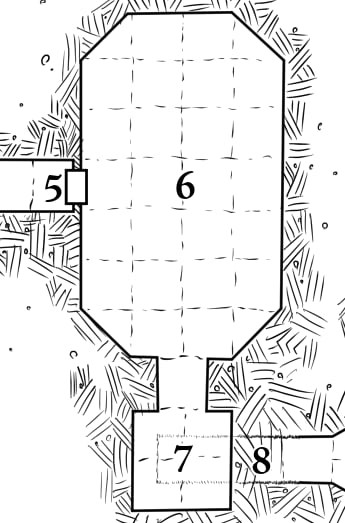
\includegraphics[width=\columnwidth]{pics/map_5-8.jpg}
\end{center}
\subsection{6 : Fausse Tombe Royale}\label{n1:s6}
La chambre funéraire du roi des hommes-serpents et ses deux épouses.
\begin{itemize}
  \item Salle de 12m sur 21m, 2.5m de haut
  \item Sent la \textbf{poussière}, \textbf{l'os} et le \textbf{moisi}
  \item Roche taillée grossièrement
  \item Fresques délitées de paysages.
  \item \textbf{3 cercueils de bois} long du mur nord
  \begin{itemize}
    \item Peints: hommes serpents endormis.
    \item Celui du milieu plus volumineux
    \item Contiennent chacun un \textbf{\nameref{monster:s6}}
    \item Attaquent dès que leur repos est troublé
  \end{itemize}
\end{itemize}



%\begin{highlight}
%\textbf{Leçons :} il y a des passages secrets.
%Ils sont associés aux statues.
%Il pourrait s'agir d'une fausse tombe.
%Tout au long de ce donjon, les statues sont synonymes de passages secrets et de trésors.
%\end{highlight}
\chapter{Niveau 2 : La Tombe Supérieure}\label{n2}
\section{Structure}
Cette section est toujours linéaire, mais avec plus de pièces annexes et quelques dangers environnementaux.
Le chemin "vers l'avant" est toujours clair, mais les salles annexes sont tentantes.
C'est ici que les leçons du Niveau 1 sont évaluées et mises en pratique.

Cet étage devrait prendre 2 ou 3 sessions à explorer, et peut requérir un trajet de retour à la civilisation pour faire le plein.


\section{Zones Thématiques}
\subsection{La Vraie Tombe}
\begin{itemize}
  \item Représente le pouvoir et les menaces implicites.
  \item Des statues veillent.
  \item Des choses tressaillent dans leurs cercueils scellés.
  \item Des lézards géants vous traquent dans l'obscurité, des sorciers immortels proposent des pactes indicibles et d'invincibles mucus morts-vivants serpentent à votre poursuite.
\end{itemize}

Décrivez cette zone avec des mots comme "énorme", "menaçant" et "froid".

C'est l'\oe uvre d'une civilisation bien plus ancienne, sage et cruelle que celle des PJ.
Plus ils s'enfoncent profondément, plus la tension devrait les rendre nerveux.
\vfill
\subsection{Le Gouffre}
Incarne l'inconnu, et ses promesses.
Il pourrait y avoir n'importe quoi en bas
\begin{itemize}
  \item Le centre de la Terre;
  \item Des hommes-serpents vivant toujours paisiblement dans les profondeurs
  \item etc.
\end{itemize}
C'est la toile vierge du module, sur laquelle le MJ peut venir ajouter ce que bon lui semble.

Décrivez le gouffre avec des mots comme \emph{"sans fond"}, \emph{"vertigineux, comme si le monde entier s'écroulait"} et \emph{"résonnant de lointains mais persistants échos, si vous êtes patients"}.

Les PJ ne devraient pas vouloir passer plus de temps que nécessaire au bord de l'abîme.


\ifmulticolEnd
\begin{center}
  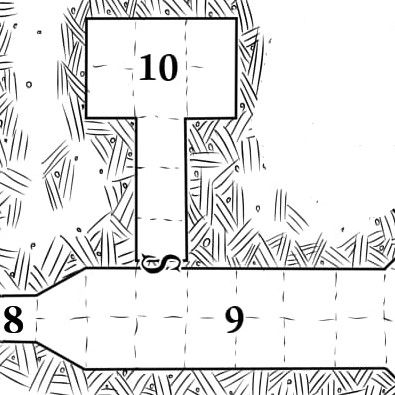
\includegraphics[width=0.6\linewidth]{pics/map_8-10.jpg}
\end{center}
\ifmulticolStart

\subsection{8 : Passage Secret}\label{n2:s8}
\begin{itemize}
  \item 9m de long sur 3m, 1.5m de haut
  \item Directement sous \textbf{\nameref{n1:s7}}
  \item \'Etroite alcôve s'élargissant sur \textbf{\nameref{n2:s9}}
  \item Sent le \textbf{moisi},et la \textbf{pierre humide}
  \item \textbf{Roche taillée finement}, mais gâchée par des fissures causées par l'eau.
  \item Flaques au sol.
\end{itemize}

\subsection{9 : Hall aux Statues}\label{n2:s9}
Un long et large couloir.
\begin{itemize}
  \item 21m de long sur 6m, 5m de haut
  \item Sent le \textbf{moisi},et la \textbf{pierre humide}
  \item Mince filet d'eau coule vers l'est
  \item Six énormes \textbf{statues d'hommes-serpents} en armes et armures
  \begin{itemize}
    \item Regard dédaigneux
    \item 1\iere{} à gauche : légèrement désalignée
    \item déplacée, révèle \textbf{\nameref{n2:s10}}
  \end{itemize}
\end{itemize}

\vfill
\subsection{10 : Salle de Garde Secrète}\label{n2:s10}
Cette pièce fut autrefois une salle de garde secrète pour les assassins du temple.

\begin{itemize}
  \item Salle de 9m sur 6m, 3m de haut
  \item Sent le \textbf{bois pourrissant},et le \textbf{tissu putréfié}
  \item Vide et sombre.
  \item Les meubles ont pourri jusqu'à se désagréger.
  \item Deux guisarmes sont toujours utilisables
  \item Une icône religieuse en argent valant 50 PO.
\end{itemize}

\vfill\pagebreak
\subsection{11 : Atrium des Tombes}\label{n2:s11}
\begin{itemize}
    \item Pièce \textbf{octogonale}, avec une ouverture au sud ouest, des portes sur les autres côtés
    \item 18m sur 18m, 5m de haut
    \item Sent le \textbf{réglisse} et la \textbf{décomposition}
    \item Bordée de statues scrutatrices d'hommes-serpents
    \item Porte Sud-Est en bois
    \item Porte Est en pierre finement ouvragée: gravures de serpents pleuvant des cieux.
    \item Autres scellées par d'épaisses portes de pierre
    \begin{itemize}
        \item tombe aisément en faisant levier
    \end{itemize}
    \item Au centre \textbf{bassin empli d'eau} de 2m de diamètre
    \begin{itemize}
        \item Eau \textbf{sombre} et \textbf{huileuse} qui sent la \textbf{réglisse}
        \item Profond de 3m
        \item 2 \textbf{\nameref{monster:s11}}, bondissent et attaquent quiconque s'approche
    \end{itemize}
\end{itemize}



Toucher l'eau ne déclenche pas de pourriture momifiante, mais la boire ou la mettre en contact avec une blessure ouverte, si.

Le bassin contient :
\begin{enumerate}
    \item Une \textbf{tête de momie} en furie qui a sombré depuis longtemps dans la folie ;
    \item Une lourde \textbf{chaîne d'or} valant 350 PO ;
    \item Un \textbf{anneau magique} en argent ;
    \item Un \textbf{outil magique} au choix du MJ ou aléatoire, ou 2d10x10 PO de joaillerie.
\end{enumerate}

\begin{center}
  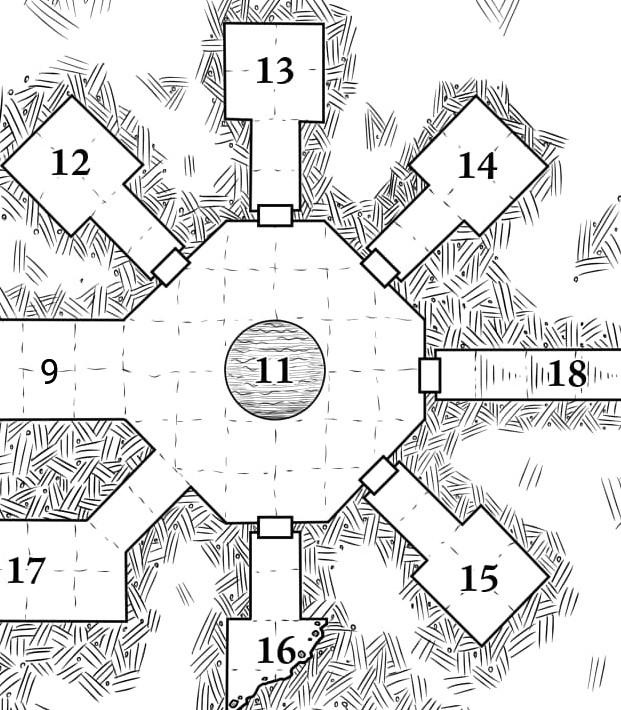
\includegraphics[width=0.9\linewidth]{pics/map_11-18.jpg}
\end{center}

\vfill

\begin{highlight}[Anneau d'argent : bague de vision]
Enfilée au doigt, l'un des yeux du porteur jaillit de son orbite, et devient dur comme du verre.
L'\oe il voit toujours normalement.
\end{highlight}


\subsection{12 : Tombe de Xisor le Vert}\label{n2:s12}
\subsubsection{Passage}
\begin{itemize}
    \item Odeur d'\textbf{ozone}
    \item \textbf{Dalle piégée} dans le passage
    \item Active un sort d'\textbf{éclair}, vers l'entrée du couloir (4d6 dégâts, 2d6 si sauvegarde Sorts)
    \item Activé une seule fois
    \item Tiré depuis une \textbf{plaque d'électrum} dans le mur (100PO)
\end{itemize}
\subsubsection{Tombe}
\begin{itemize}
  \item Salle de 6m sur 6m, 3m de haut
  \item Sent les \textbf{épices d'embaumement}
  \item 1 \textbf{cercueil de pierre}
\end{itemize}
Un parchemin de sort (venin oculaire, ou autre sort basé sur le venin) se trouve dans le
cercueil de Xisor.

%\vfill\columnbreak
\subsection{13 : Tombe de Sparamantur}\label{n2:s13}
\begin{itemize}
  \item Salle de 6m sur 6m, 3m de haut
  \item Porte de pierre brisée
  \item Passage partiellement \textbf{effondré}
  \item Si excavation : \textbf{sons d'agitation} de l'autre côté
  \item \textbf{\nameref{monster:s13}} attaque à vue
  \begin{itemize}
    \item Squelette homme-serpent
  \end{itemize}
  \item Ses ornements funéraires valent 100 PO
\end{itemize}

\subsection{14 : Tombe de Franbinzar}\label{n2:s14}
\begin{itemize}
    \item Salle de 6m sur 6m, 3m de haut
    \item Sent le \textbf{goudron} et la \textbf{décomposition}.
    \item Tombe décorée de \textbf{peintures} et \textbf{gravures obscènes}
    \item \textbf{Cercueil de pierre :} restes de \textbf{\nameref{monster:s14}} (Pudding Noir)
    \begin{itemize}
      \item \textbf{Ouverture :} attaque
      \item \textbf{Trésor :} copies d'argile, mais 200 PO d'anneaux sont noyés dans sa masse
    \end{itemize}
\end{itemize}

Si Franbinzar a été libéré, il est ajouté à la Table des \textbf{\nameref{monster:n3:errants}} à la place d'un des présages.

\vfill\columnbreak

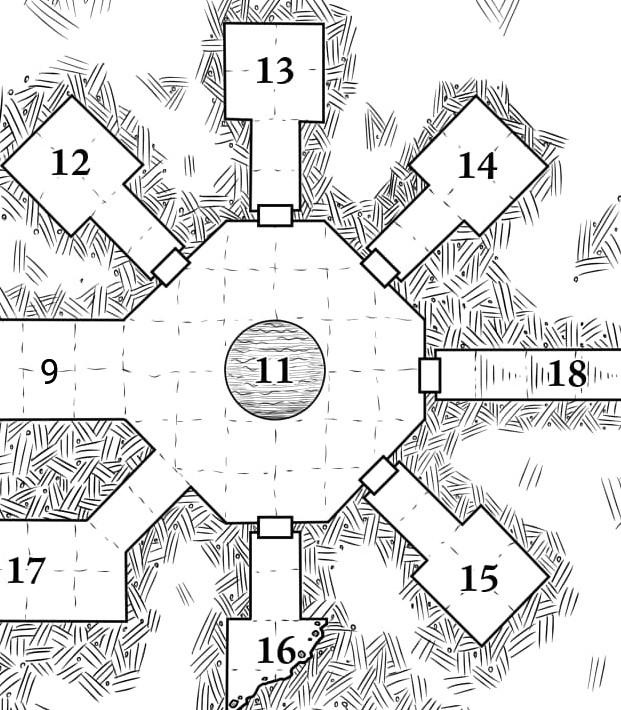
\includegraphics[width=\linewidth]{pics/map_11-18.jpg}

\subsection{15 : Sacristie}\label{n2:s15}
Cette pièce était utilisée par les prêtres de la tombe supérieure.
\begin{itemize}
  \item Salle de 6m sur 6m, 3m de haut
  \item Sent le \textbf{bois pourrissant} et la \textbf{poussière}.
\end{itemize}
Elle contient :
\begin{itemize}
    \item Trois lits,
    \item Des étagères vermoulues,
    \item Une icône religieuse de dieu-serpent en argent et émeraude (200 PO)
    \item Parchemins en langue inconnue (témoignent de la folie des momies emprisonnées).
          Éparpillés au sol.
          \begin{itemize}
            \item l'un contient le nom de la \textbf{\nameref{monster:n3:succube}} piégée en \textbf{\nameref{n3:s32}}
          \end{itemize}
\end{itemize}

\subsection{16 : Tombe Inachevée}\label{n2:s16}
\begin{itemize}
  \item Salle de 6m sur 3m, 2m de haut
  \item Salle à moitié creusée
  \item Des outils d'excavation rouillent au sol..
\end{itemize}

\vfill

\subsection{17 : Soldats d'Argile}\label{n2:s17}
\begin{itemize}
    \item Salle de 12m sur 6m, 3m de haut
    \item 3 rang de 6 \textbf{statues d'argile} de soldats hommes-serpents à taille réelle:
    \begin{itemize}
      \item Apparence froide et sinistre
      \item Leurs épées sont rouillées et inutiles
      \item Creuses mais vides
    \end{itemize}
    \item Sous la statue au Sud-ouest : passage secret vers 38 : le Hall du Basilic (p. 9)
\end{itemize}


\newpage
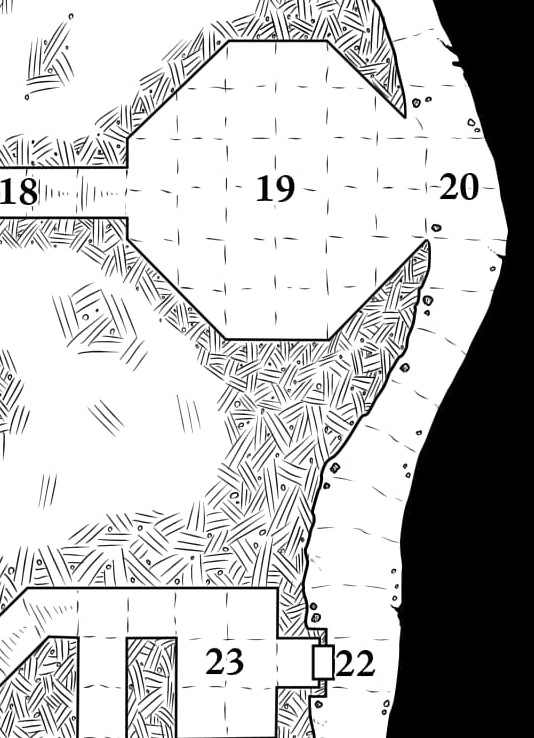
\includegraphics[width=\columnwidth]{pics/map_18-23.jpg}

\subsection{18 : Escaliers}\label{n2:s18}
\begin{itemize}
  \item Couloir de 15m de long, 3m de large et 3m de haut
  \item Air froid, \textbf{silence} total.
  \item Des \textbf{escaliers} s'enfoncent dans les ténèbres.
  \item Une légère brise se fait sentir.
\end{itemize}

La troisième volée de marches est piégée.

\begin{highlight}[Piège]
Dès qu'un poids est appliqué sur la marche
\begin{itemize}
    \item Les marches basculent pour former une rampe de roche lisse
    \item Des épieux jaillissent du sol en bas de l'escalier (1D8 dégâts, 1D4 si sauvegarde Mort)
    \item Se réarme après 5 rounds
\end{itemize}
\end{highlight}

\vfill

\subsection{19 : Arène du Gardien Cobra}\label{n2:s19}
\begin{itemize}
    \item Même forme et taille que \nameref{n2:s11}
    \item Pièce \textbf{octogonale}, avec une \textbf{grande ouverture} à l'est
    \item 18m sur 18m, 5m de haut
    \item \textbf{Arène} froide,
    \item Murs couverts de boucliers divers (des tribus vaincues par les hommes-serpents)
    \begin{itemize}
      \item 5 sont fonctionnels, les autres pourris
      \item 20 PO récupérables en les désassemblant (décorations en argent)
    \end{itemize}
    \item Au centre une statue de pierre en forme de cobra
    \begin{itemize}
      \item \textbf{\nameref{monster:s19}} attaque à vue
    \end{itemize}
\end{itemize}

\subsection{20 : Gouffre et Chemin}\label{n2:s20}
\begin{itemize}
  \item \'Etroit chemin (3m) 24 m jusqu'à \textbf{\nameref{n3:s22}}
  \item \textbf{Glissant} : course ou saut : chute dans le gouffre.
  (sauvegarde contre la mort +5 annule)
  \item \textbf{Gouffre} abyssal à l'est
  \begin{itemize}
    \item large de 18m
    \item mur opposé non visible
  \end{itemize}
\end{itemize}
Si le groupe se met les gobelins fongiques à dos, ils tendent toujours une embuscade ici.
Les gobelins sont collants et ignorent le sol glissant

\subsection{21 : Patelles des Donjons}\label{n2:s21}
\begin{wrapfigure}{l}{0.3\linewidth}
  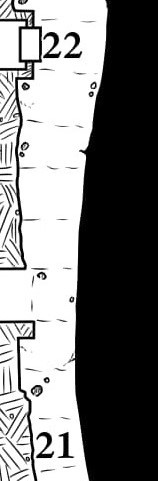
\includegraphics[width=\linewidth]{pics/map_21-22.jpg}
\end{wrapfigure}
Chemin couvert de \textbf{patelles des donjons}:
\begin{itemize}
  \item mollusques à coquille de pierre
  \item \textbf{Contact :} paralysie 1D4 heures (sauvegarde paralysie annule)
  \item \textbf{Paralysé :} dévoré en 1D4 heures
  \item Connu si expérience de donjon
\end{itemize}








\chapter{Niveau 3 : La Tombe Inférieure}\label{n3}
\section{Structure}
Il y a deux chemins principaux "horizontaux" et trois "verticaux".
Le donjon bifurque et reboucle.

Il est possible de remonter à la surface comme de plonger plus profond.
Ou même de revenir de là où l'on est parti.
Cet étage est indubitablement plus dangereux que les précédents.

La diplomatie et le troc font également leur apparition, de même que les \nameref{monster:n3:errants}.
Vous pouvez explorer les niveaux 1 et 2 à votre rythme, mais passer trop de temps au Niveau 3 revient à prendre des risques inconsidérés.

La conclusion de cet étage est ouverte : vous pouvez ajouter du contenu pour étendre ce donjon autant que vous le souhaitez.
Arrivé là, si vous êtes un nouveau MJ ou débutant en jeux OSR, vous devriez être prêt à écrire votre propre donjon.

\section{Zones Thématiques}
\subsection{Les Terriers Gobelins}
Les Gobelins Fongiques sont le miroir des PJ, leur opposé.
Ils se complaisent dans la crasse, revivent sans cesse et commettent toujours les mêmes erreurs.
Ils sont affamés, stupides, superstitieux et meurtriers, mais néanmoins attachants.
Les terriers sont l'irruption d'un barbarisme bruyant et enthousiaste dans la civilisation froide et moribonde.



Décrivez les terriers tant par le bruit que par l'odeur.
Ça pue.
Vous allez puer si vous vous attardez ici, et la Tombe des Rois Serpents n'est pas pourvue de bains.
Des petits yeux de gobelins dans la pénombre.
Des dents cliquetantes et des couteaux aiguisés.

\ifmulticolEnd
\begin{center}
  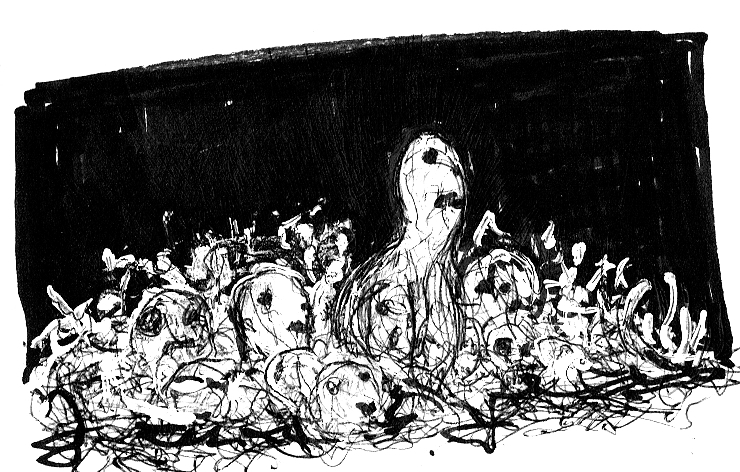
\includegraphics[width=0.5\columnwidth]{pics/goblin_pit.jpg}
\end{center}
\ifmulticolStart

\vfill
\pagebreak

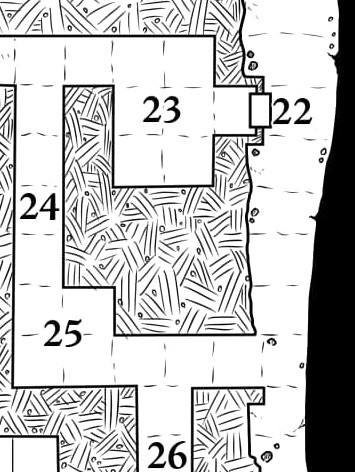
\includegraphics[width=\columnwidth]{pics/map_22-25.jpg}
\subsection{22 : Porte de Pierre}\label{n3:s22}
\begin{itemize}
  \item Enfoncée d'1,50m dans le mur
  \item Maintenue fermée par une lourde barre de pierre côté gouffre.
  \item En arrivant par l'autre côté, la porte ne peut être ouverte sans être détruite.
  \item \textbf{Piège :}
  \begin{itemize}
    \item Même que \nameref{n1:s5}
    \item Marteau vers l'extérieur :
    \begin{itemize}
      \item 1D6 dommage \textbf{puis :} (sauvegarde contre la mort +2 annule)
      \item Poussé dans le gouffre (sauvegarde contre la mort annule)
    \end{itemize}
  \end{itemize}
\end{itemize}

\subsection{24 : Couloir}\label{n3:s24}
\begin{itemize}
  \item Couloir de 3m sur 12m, 3m de haut
  \item Sent légèrement l'\textbf{acide}
  \item Bruits de \textbf{claquements humides}.
  \item Descend en pente douce vers le sud.
  \item \textbf{\nameref{monster:n3:squelgel}} au sud attiré par le bruit
\end{itemize}

\vfill

\subsection{23 : Salle Cérémonielle}\label{n3:s23}
\begin{itemize}
  \item Salle de 6m sur 9m, 3m de haut
  \item Sent les \textbf{champignons séchés} et la \textbf{poussière}.
  \item Bancs au centre
  \item Anciennes tapisseries aux murs
  \item Fontaine asséchée (mur sud) :
  \begin{itemize}
    \item Résidus d'or (10PO) sur espace plat au milieu
  \end{itemize}
\end{itemize}

Utilisée autrefois par les prêtres hommes-serpents pour se préparer et méditer.

Les gobelins ont arraché la statue d'or qui ornait la fontaine pour la cacher dans leur salle du trône.

\subsection{25 : Fosse Piégée}\label{n3:s25}
\begin{itemize}
  \item Salle de 6m sur 6m, 3m de haut
  \item Air \textbf{froid}
  \item Carrelage de dalles :
  \begin{itemize}
    \item certaines cassées
    \item une manquante
  \end{itemize}
  \item \textbf{Piège :}
  \begin{itemize}
    \item Corniche large de 30 cm le long des murs, \textbf{sûre}
    \item Autres carreaux ne sont soutenus que par de fines barres de métal
    \item Pied dans la zone centrale :
    \begin{enumerate}
      \item \textbf{Chute :} 1D6 dégâts (sauvegarde contre la mort annule)
      \item \textbf{Empalé} par les pics au fond : 1D6 dégâts (sauvegarde contre la mort annule)
    \end{enumerate}
  \end{itemize}
\end{itemize}

La fosse contient plusieurs squelettes d'humains normaux, ainsi qu'un anneau d'or valant 20 PO.

Les gobelins remplacent les dalles chaque jour : ils utilisent le piège pour capturer leurs proies.

\vfill\pagebreak

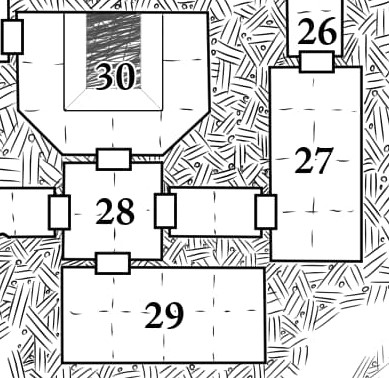
\includegraphics[width=\columnwidth]{pics/map_26-30.jpg}
\subsection{26 : Couloir}\label{n3:s26}
\begin{itemize}
  \item Couloir de 3m sur 6m, 3m de haut
  \item Mène à porte verrouillée :
  \begin{itemize}
    \item \textbf{Serrure aisée :} capacité voleur x2
    \item \textbf{Corrodée :} considérer comme une porte bloquée
  \end{itemize}
\end{itemize}

\subsection{27 : Salle des Esclaves}\label{n3:s27}
\begin{itemize}
  \item Salle de 6m sur 12m, haute de 3m
  \item Air \textbf{chaud et vicié}.
  \item Taches de sang et roche usée
  \item \textbf{Sifflement} constant au sud-est.
  \item \textbf{Entraves rouillées} au sol.
  \begin{itemize}
    \item Se referment aux jambes si à moins de 30cm
    \item Rouille : Brisées avec test de force
  \end{itemize}
\end{itemize}


\subsection{28 : Dôme}\label{n3:s28}
\begin{itemize}
  \item Salle de 6m sur 6m, haute de 6m
  \item Air \textbf{chaud et vicié}.
  \item \textbf{Sifflement} constant au nord.
  \item Plafond : \textbf{Dôme},  fresques d'hommes-serpents triomphants
  \item Porte au milieu de chaque mur.
  \item Porte sud verrouillée :
  \begin{itemize}
    \item Clef est au cou du Basilic (p. 14)
    \item Trop épaisse pour être brisée
  \end{itemize}
  \item Porte de pierre brisée à l'est.
  \item Porte de pierre entrouverte vers le nord.
\end{itemize}

\vfill

\subsection{29 : Salle du Trésor}\label{n3:s29}
\begin{itemize}
  \item Salle de 12m sur 6m, haute de 6m
  \item Contient tout ce que le MJ jugera bon de mettre au fond d'un donjon. [2000 PO au moins]
\end{itemize}

\subsection{30 : Fosse Sacrificielle}\label{n3:s30}
\begin{itemize}
  \item Salle de 12m sur 9m, haute de 6m
  \item Air vicié,
  \item \textbf{Flamme orangée} au nord, au fond d'une fosse profonde de 5m  aux parois en pente.
  \item Feu est alimenté par du gaz naturel acheminé depuis une antique mine perdue dans les tréfonds
  \item Chemin large de 60 cm borde le trou
  \item \textbf{Os carbonisés} couvrent le fond
  \item \textbf{Coulures d'or} sont visibles autour de la flamme
  \item \textbf{Pierres précieuses} couvertes de carbone (500 PO en tout) scintillent dans la lueur orangée du feu
  \item Si PJ entrent dans la fosse :
  \begin{itemize}
    \item -1D6 CON (temporaire, sauvegarde poison annule)
    \item 0 CON : inconscient, glisse jusqu'à la flamme :  2d6 dégâts de feu par round
  \end{itemize}
\end{itemize}

\vfill
\pagebreak


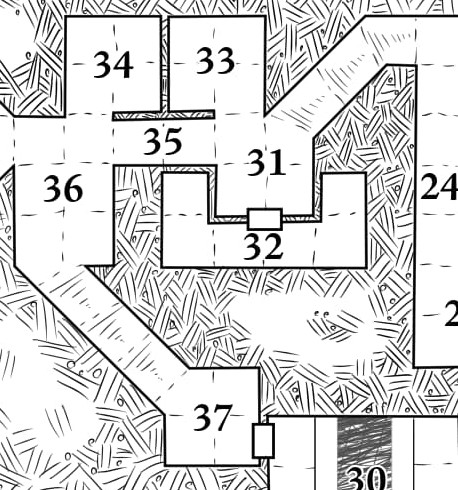
\includegraphics[width=\columnwidth]{pics/map_31-37.jpg}

\subsection{31 : Hall Gardé}\label{n3:s31}
\begin{itemize}
  \item Salle de 6m sur 6m, haute de 3m
  \item Sent la \textbf{poussière}
  \item Faible \textbf{cliquetis de chaîne} dans le lointain.
  \item Deux \textbf{statues de gardes} hommes-serpents aux coins sud
  \begin{itemize}
    \item Incroyablement \textbf{réalistes}
    \item Bien plus fines que tous les autres reliefs de la tombe
  \end{itemize}
\end{itemize}

Les statues sont des hommes-serpents pétrifiés, placés ici en guise de punition.
S'ils sont dé-pétrifiés, ils entrent dans une rage noire pendant 10 minutes, puis sombrent dans le désespoir.

Les statues peuvent se vendre 500 PO chacune dans une grande ville, ou 10 fois plus à un mage capable de reconnaître leur véritable nature.

\vfill

\subsection{32 : Salle d'Invocation}\label{n3:s32}
\begin{itemize}
  \item Salle de 12m sur 6m, haute de 3m, en forme de U
  \item Odeur de \textbf{vieux vin}, \textbf{papier brûlé} et \textbf{pourriture fongique}
  \item \'Enorme pile de débris bloque la porte.
  \begin{itemize}
    \item 30 minutes à déblayer,
    \item Très Bruyant
  \end{itemize}
  \item côté ouest, un \textbf{\nameref{monster:n3:succube}}
  \begin{itemize}
    \item \textbf{Non hostile}
    \item Prétend avoir été capturé par les gobelins et gardé prisonnier
    \item \textbf{Entravé} au pied (illusion)
    \item Au centre d'un cercle de confinement (difficile à voir)
    \begin{itemize}
      \item Brisé si franchi
    \end{itemize}
  \end{itemize}
  \item Petit \textbf{autel}
  \item 2 \textbf{bols en or} (150 PO chacun)
  \item \textbf{Dague magique} +1
  \item \textbf{Serpent de pierre} sinueux
  \begin{itemize}
    \item Magique
    \item Permet d'ouvrir la porte de \nameref{n3:s46}
  \end{itemize}
\end{itemize}

La pièce s'avère être une ancienne chambre d'invocation.
Baltoplate a été invoqué par les hommes-serpents pour répondre à leurs questions sur les enfers abyssaux.


\subsection{33 : Autel}\label{n3:s33}
\begin{itemize}
  \item Salle de 6m sur 6m, haute de 3m
  \item Sent légèrement l'\textbf{acide}.
  \item \textbf{Statue menaçante} à tête de cobra.
  \begin{itemize}
    \item Percée à sa base de deux trous assez larges pour laisser passer un bras humain
    \item \textbf{A du jeu :} peut pivoter.
    \item Sens anti-horaire : gaz empoisonné (1D6 dégâts, sauvegarde poison annule).
    \item Sens horaire : [2d1000 + 100 PO].
  \end{itemize}
\end{itemize}

\vfill
\pagebreak

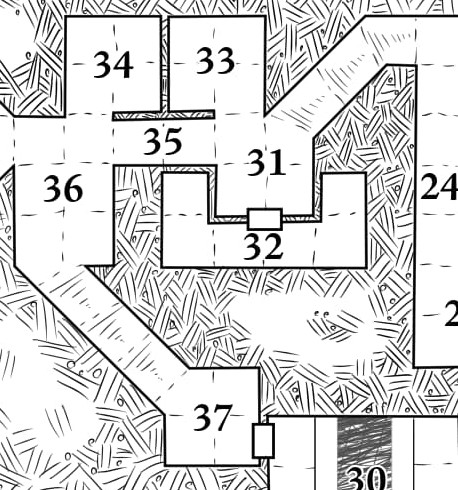
\includegraphics[width=\columnwidth]{pics/map_31-37.jpg}
\subsection{34 : Zone de Repos des Prêtres}\label{n3:s34}
\begin{itemize}
  \item Salle de 6m sur 6m, haute de 3m
  \item Odeur de \textbf{sang desséché}, de \textbf{tissus pourrissants} et de \textbf{champignons défraîchis}.
  \item Porte de bois a pourri sur place.
  \item 5 Coussins déchiquetés, maculés de sang
  \item \textbf{3 \oe ufs de pierre }
  \begin{itemize}
    \item Magiques
    \item Enduits de sang : chauffe (bouillotte) 8 heures
  \end{itemize}
\end{itemize}

\subsection{35 : Corridor Piégé}\label{n3:s35}
\begin{itemize}
  \item Couloir de 6m sur 3m, haut de 3m
  \item Sent la \textbf{poussière}.
  \item \textbf{4 sillons au plafond} évoquant le corps d'un serpent
  \item \textbf{Bandes de dalles} serpentent au sol.
  \begin{itemize}
    \item Marcher dessus : déclenche
    \item 4 pendules tranchants surgissent du plafond : 1D6 dégâts (sauvegarde mort annule)
    \item Pendant 3 round : si mouvement, doit esquiver un pendule
    \item Round 4 : tout s'écroule. 2D6 de dégâts (sauvegarde mort $\textonehalf$ dégâts)
  \end{itemize}
\end{itemize}

\vfill

\subsection{36 : Vestibule}\label{n3:s36}
\begin{itemize}
  \item Salle de 6m sur 9m, haute de 5m
  \item Sent le \textbf{tissu pourrissant}.
  \item Tintement de chaîne à l'ouest.
  \item Tentures partiellement pourries jonchent le sol
  \item Dallage à motifs géométriques.
  \item Se plaquer au mur ouest permet de se cacher du \textbf{\nameref{monster:n3:basilic}}.
  \item Couloir en pente vers le sud-est.
\end{itemize}


\subsection{37 : Fosse Piégée}\label{n3:s37}
\begin{itemize}
  \item Salle de 6m sur 6m, 3m de haut
  \item Air \textbf{froid}
  \item Carrelage de dalles :
  \begin{itemize}
    \item certaines cassées
    \item une manquante
  \end{itemize}
  \item \textbf{Piège :}
  \begin{itemize}
    \item Corniche large de 30 cm le long des murs \textbf{sûre}
    \item Autres carreaux ne sont soutenus que par de fines barres de métal
    \item Pied dans la zone centrale :
    \begin{enumerate}
      \item \textbf{Chute :} 1D6 dégâts (sauvegarde contre la mort annule)
      \item \textbf{Empalé} par les pics au fond : 1D6 dégâts (sauvegarde contre la mort annule)
    \end{enumerate}
  \end{itemize}
  \item Fosse vide
\end{itemize}

\vfill

\pagebreak

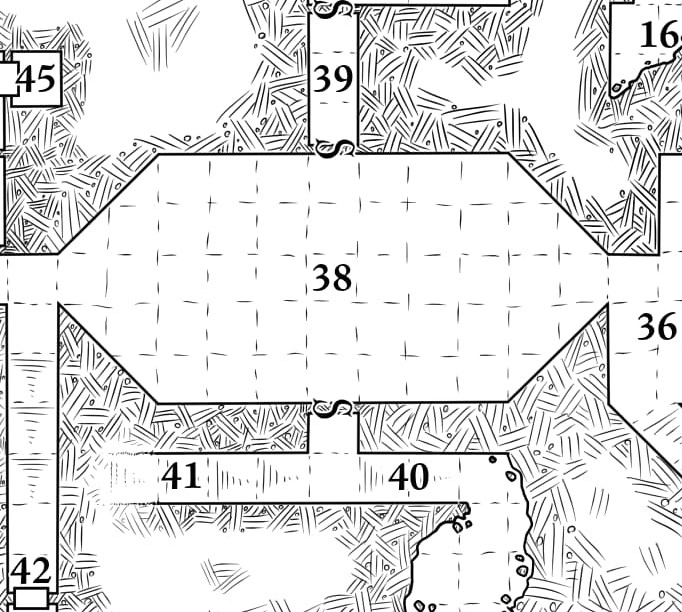
\includegraphics[width=\columnwidth]{pics/map_38-42.jpg}

\subsection{38 : Hall du Basilic}\label{n3:s38}
\begin{itemize}
  \item Grande salle de 34m sur 17m, haute de 15m
  \item Creusée à même la roche
  \item Air stagnant
  \item Tintements de chaîne
  \item Respiration à peine perceptible (\textbf{\nameref{monster:n3:basilic}})
  \item \textbf{8 piliers de roche}, certains détruits.
  \item \textbf{Statues de pierre} (araignées, gobelins, chauve-souris) détruites et parsemant le sol.
  \item Statues taillés avec une incroyable précision
  \item Mosaïques d'hommes-serpents triomphants sur les murs.
\end{itemize}

\subsection{39 : Passage Secret}\label{n3:s39}
\begin{itemize}
  \item Couloir de 3m sur 12m, 1.5m de haut
  \item Air stagnant, nuages de poussière.
  \item Taillé  à même la roche
  \item La porte devrait être invisible mais la mosaïque la cachant est endommagée et la \textbf{révèle}
  \item Mène en \textbf{\nameref{n2:s17}}
\end{itemize}


\subsection{40 : Passage Secret}\label{n3:s40}
\begin{itemize}
  \item Couloir de 3m sur 3m, 1.5m de haut
  \item Air aigre, relents immondes.
  \item \textbf{Intact}, caché par une mosaïque.
  \begin{itemize}
    \item \textbf{Difficile} à détecter
    \item Même principe que celle au nord : \textbf{localisable}
  \end{itemize}
  \item Murs lisses et soigneusement taillés
  \item Sol couvert de \textbf{ détritus gobelins}.
\end{itemize}

\subsection{41 : Escalier vers la Surface}\label{n3:s41}
\begin{itemize}
  \item Couloir de 10m sur 1m, 2.5m de haut
  \item Terreux, humide.
  \item Émerge entre les racines d'un arbre.
\end{itemize}

\subsection{42 : Porte en Cylindre}\label{n3:s42}
  \begin{itemize}
    \item Au bout d'un corridor de 3m sur 18m, 3m de haut
    \item Couloir en pente
    \item \textbf{Cylindre de roche} taillé d'une alcôve
    \begin{itemize}
      \item Peut accueillir deux personnes.
      \item Pivote dans les deux sens
      \item \textbf{Sens anti-horaire :} l'alcôve arrive face à des lances jaillissant de la roche
      pour transpercer les occupants (1d6 dégâts par round).
      \item \textbf{Sens horaire :} autel avec idole de pierre portant 2 bols en or (100 PO chaque).
      \item \textbf{180 degrés :} débouche sur \nameref{n3:s47}
    \end{itemize}
\end{itemize}

\vfill\pagebreak
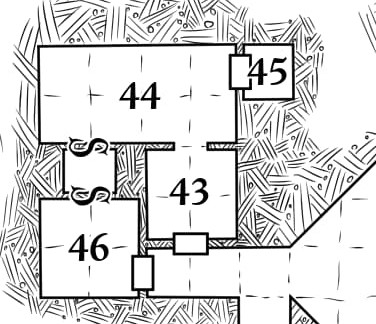
\includegraphics[width=\columnwidth]{pics/map_43-46.jpg}

\subsection{43 : Antichambre de Xiximantre}\label{n3:s43}
\begin{itemize}
  \item Salle de 6m sur 6m, 5m de haut
  \item Relents âcres, milles odeurs
  \item Taillée à même la roche
  \item Bas-reliefs de pierre noire.
  \item Lampes magiques violacées incrustées dans les murs
  \item Présence de  \textbf{\nameref{monster:n3:xiximanter}}
\end{itemize}

\subsection{44 : Réserve à Ingrédients}\label{n3:s44}
\begin{itemize}
  \item Salle de 12m sur 6m, 5m de haut
  \item Relents âcres, milles odeurs
  \item Lampes magiques violacées incrustées dans les murs
  \item Barils, caisses, cercueils, flacons, bottes d'herbes.
  \begin{itemize}
    \item Une fiole contient du safran en poudre (2000 PO)
    \item Une petite bouteille renferme  1d10 graines d'une espèce de plante à présent disparue (300 PO chacune)
  \end{itemize}
  \item Six oubliettes à couvercles de bronze sont incrustées dans le sol
  \item Une contient  1d10 Gobelins Fongiques.
  \item Passage secret derrière les caisses
\end{itemize}

Xiximantre ne cédera rien de son stock à moins d'obtenir en échange des ingrédients d'encore plus grande rareté ou valeur

\vfill

\subsection{45 : Laboratoire à Potions}\label{n3:s45}
\begin{itemize}
  \item Salle de 3m sur 3m, 3m de haut
  \item Lampes magiques violacées, bouillonnement,
  \item Éprouvettes alchimiques, verrerie poussiéreuse et étagères luisantes de magnifiques flacons.
  \item Porte de fer verrouillable.
  \item À peine assez de place pour travailler.
  \item Sur les étagères :
  \begin{itemize}
    \item 2 potions de mutation de sort
    \item 1 potion d'immortalité modérée (1d100 + 20 années de vie naturelle supplémentaires)
    \item 1 potion de poison indétectable (aucun goût mais tue (pas de jet de sauvegarde) en 1 minute)
    \item 2 potions de soin
    \item 1d10 + 10 potions aléatoires
  \end{itemize}
\end{itemize}

Xiximantre n'autorisera pas les PJ à y accéder à moins qu'ils n'acceptent de devenir ses apprentis (ou victimes)

Ses potions les plus puissantes prennent des décennies à élaborer.
Il est prêt à échanger ses concoctions contre des créatures vivantes, sorts, ingrédients rares et apprentis.
Il n'acceptera ni monnaie ni trésors.

Si les aventuriers transportent ouvertement des objets pillés dans la tombe, cela éveillera ses soupçons et il tentera de les empoisonner, capturer ou manipuler.

\subsection{46 : Salle du Trône}\label{n3:s46}
\begin{itemize}
  \item Salle de 6m sur 6m, 6m de haut
  \item Sent la poussière et les copeaux de métal.
  \item La porte est faite de \textbf{serpents de pierre} entremêlés.
  \begin{itemize}
    \item L'un est manquant, en \textbf{\nameref{n3:s32}}.
    \item Si remis en place, la porte glisse et s'ouvre silencieusement
  \end{itemize}
  \item Murs de roche rouge, ornée d'ors et de \textbf{miroirs}
  \item Murs décorés d'écailles joliment gravées.
  \begin{itemize}
    \item 8 miroirs de la taille d'une main dressés sur des présentoirs en bois : 100 PO chaque
    \item trône : 2500 PO.  3 personnes pour le soulever
  \end{itemize}
  \item \textbf{Passage secret} derrière une tenture pourrissante.
\end{itemize}

Si les PJ utilisent le passage secret, le sorcier sera surpris, ainsi que furieux s'ils ne parviennent pas à donner une excuse plausible.

\vfill\pagebreak
\ifmulticolEnd
\begin{center}
  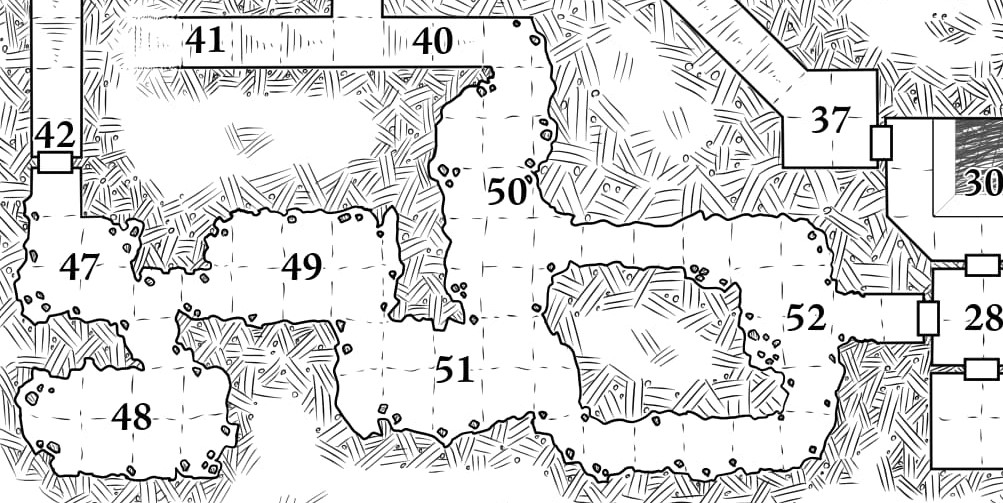
\includegraphics[width=\linewidth]{pics/map_47-52.jpg}
\end{center}
\ifmulticolStart

\subsection{47 : Terrier Gobelin}\label{n3:s47}
\begin{itemize}
  \item Salle de 6m sur 6m, 1.5m de haut
  \item Empeste le graillon, les champignons, la pourriture et l'humidité.
  \item Chuchotis.
  \item Sol couvert de scarabées
  \item Des détritus jusqu'au mollet.
  \item Fouille des débris :
  \begin{itemize}
    \item 2d6 couteaux d'argent (10 PA chaque)
    \item PJ couvert de fange et guano
  \end{itemize}
  \item Stock de plumes, chiffons et bols de graisse
\end{itemize}

\subsection{48 : Fosse de Génération de Gobelins}\label{n3:s48}
\begin{itemize}
  \item Salle de 12m sur 6m, 1.5m de haut
  \item Pestilence fongique, animaux pourrissants, gobelins à demi formés.
  \item \textbf{Spectacle répugnant :} Jet de sauvegarde contre le poison ou fuite avec nausée
\end{itemize}

La fosse réincarne les âmes des gobelins fongiques morts, c'est l'une des expériences ratées de
\textbf{\nameref{monster:n3:xiximanter}}, censée apporter l'immortalité.

Aucun trésor ici, mais tant que cette salle n'est pas incendiée, le nombre de gobelins dans le donjon sera toujours \emph{"beaucoup trop de gobelins"}.

\vfill

\subsection{49 : Salle du Trône Gobeline}\label{n3:s49}
\begin{itemize}
  \item Salle de 9m sur 6m, 1.5m de haut
  \item Chuchotis, bruits de scarabées écrasés
  \item 1d6 (explosif) \textbf{\nameref{monster:n3:gob}} présents
  \begin{itemize}
    \item Mangent des chauves-souris, se battent ou vénèrent leur roi actuel
    \item Si aucun Roi : vénèrent une idole sculptée en boue et brindilles
  \end{itemize}
  \item \textbf{Couronne gobeline :} faite de bâtons et couverts tordus
\end{itemize}


\subsection{51 : Dortoir Gobelin}\label{n3:s51}
\begin{itemize}
  \item Salle de 15m sur 6m, 1.5m de haut
  \item Crasse, pourriture, chuchotis
  \item Statues grossières de boue et bâtons.
  \item \textbf{Nuit :} 1d6 (explosif) \textbf{\nameref{monster:n3:gob}}
  \item \textbf{Jour :} 3d6+10 (explosif) \textbf{\nameref{monster:n3:gob}}
  \begin{itemize}
    \item Presque \textbf{invisibles} parmi les débris.
    \item \textbf{Endormis}
    \item \textbf{Bruit :} se réveillent en 2 rounds
  \end{itemize}
\end{itemize}

\vfill
\pagebreak

\ifmulticolEnd
\begin{center}
  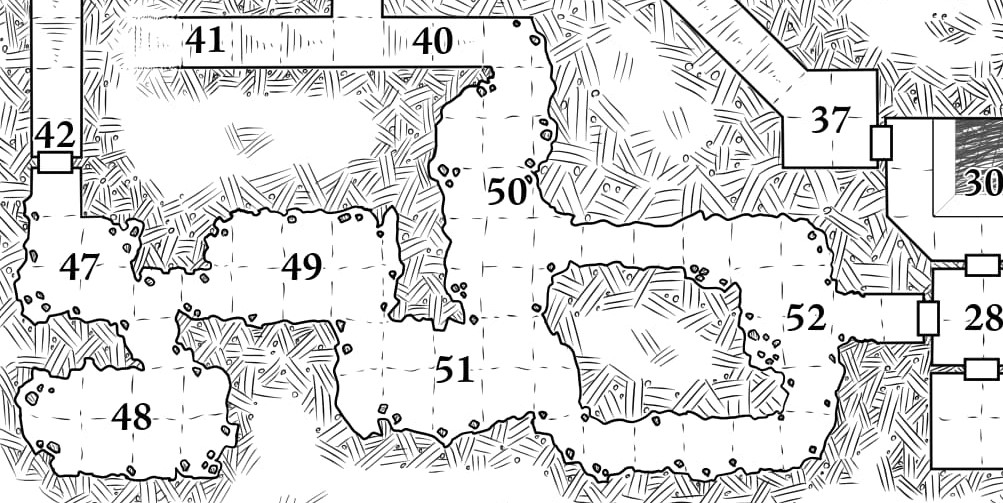
\includegraphics[width=\linewidth]{pics/map_47-52.jpg}
\end{center}
\ifmulticolStart

\subsection{50 : Fermes Gobelines}\label{n3:s50}
\begin{itemize}
  \item Salle de 6m sur 12m, 1.5m de haut
  \item Plantes en putréfaction, puanteur du fumier, spores de champignons
  \item Sol inégal
  \item Des détritus jusqu'aux genoux
  \item Les \textbf{\nameref{monster:n3:gob}} plantent tout et n'importe quoi
  \item \textbf{Fouille} (1 tour par carré de 1.5m) :
  \begin{enumerate}
    \item Un doigt et une fourchette
    \item Une dague rouillée
    \item 2D100 PO
    \item Rubis (300 PO)
    \item Des os de poulet
    \item \textbf{Couronne des rois serpents}
  \end{enumerate}
\end{itemize}

Les apothicaires et sorciers expérimentés peuvent identifier les champignons bleus poussant ici comme des concombres des donjons, capables de guérir la pétrification en 1d6 jours une fois coupés en rondelles et frottés contre la peau.

\vfill
\
\begin{highlight}[Couronne des rois serpents]
  \begin{itemize}
    \item Composée de 8 petits serpents d'or et platine entremêlés, aux yeux d'émeraude et dents de diamant
    \item 3000 PO de matériaux
    \item \textbf{Magique :}
    \begin{itemize}
      \item \textbf{Si portée :} sauvegarde contre les sorts, ou être prostré et terrifié une heure
      \item \textbf{3 échecs} consécutifs : état permanent
    \end{itemize}
  \end{itemize}
\end{highlight}

\subsection{52 : Salle de Garde des Gobelins}\label{n3:s52}
\begin{itemize}
  \item Salle de 6m sur 6m, 1.5m de haut
  \item Air vicié
  \item Pourriture en train de sécher
  \item Stock d'armes \textbf{\nameref{monster:n3:gob}}
  \begin{itemize}
    \item 2 fourches,
    \item Une pile de couverts en argent (200 PO)
    \item des douzaines de bâtons affûtés
  \end{itemize}
  \item 1 \textbf{\nameref{monster:n3:gob}} fait le guet
  \begin{itemize}
    \item Armé d'un balai
    \item \'Eloigne les \textbf{\nameref{monster:n3:squelgel}}
    \item Repousse les PJ si arrivent du \textbf{\nameref{n3:s28}}
    \item S'enfuit en hurlant si les PJ arrivent du \textbf{\nameref{n3:s28}}
  \end{itemize}
\end{itemize}


\chapter{Description des monstres}
\section{Niveau 1}
\subsection{Squelette}\label{monster:s6}
\begin{itemize}
  \item \textbf{Apparence :}
  \begin{itemize}
    \item Squelette humain muni de crocs et d'une arme rouillée.
    \item Couvert de bracelets.
  \end{itemize}
  \item \textbf{ Désirs :} protéger le reste de la Tombe des Rois Serpents et tuer tout intrus.
  \item Ne subissent que la moitié des dégâts infligés par les armes perçantes ou tranchantes.
  \item Ils craquent et cliquettent, meurtriers et implacables
\end{itemize}

\SetTblrInner{hspan=minimal, vspan=even}
\begin{osrtable}{X[2]X[1]X[1]X[2]}{0}
  \SetCell[c=4]{bg=black,fg=white} {\bfseries\large\sectionfont Statistiques} & & &\\
  \textbf{CA}          & 7 [12] & \textbf{TACO}        & 19 [0] \\
  \textbf{Attaque}     & \SetCell[c=3]{l} 1D6 (griffes) & &\\
  \textbf{Sauvegardes} & \SetCell[c=3]{l} {\small \textbf{MP}~12 \textbf{B}~13 \textbf{PP}~14 \textbf{S}~15 \textbf{SSB}~16}& &\\
  \textbf{Mouvement} & 18m    & \textbf{Moral} & 12 \\
  \textbf{DV} & 1   & \textbf{XP} & 10 \\
  \textbf{PV} (\hspace*{20pt}) & \SetCell[c=3]{l}\noindent\hdsquares{1} & &\\
  \textbf{PV} (\hspace*{20pt}) & \SetCell[c=3]{l}\noindent\hdsquares{1} & &\\
  \textbf{PV} (\hspace*{20pt}) & \SetCell[c=3]{l}\noindent\hdsquares{1} & &\\
\end{osrtable}

\vfill\
\begin{center}
  \vspace*{0.2\textheight}
  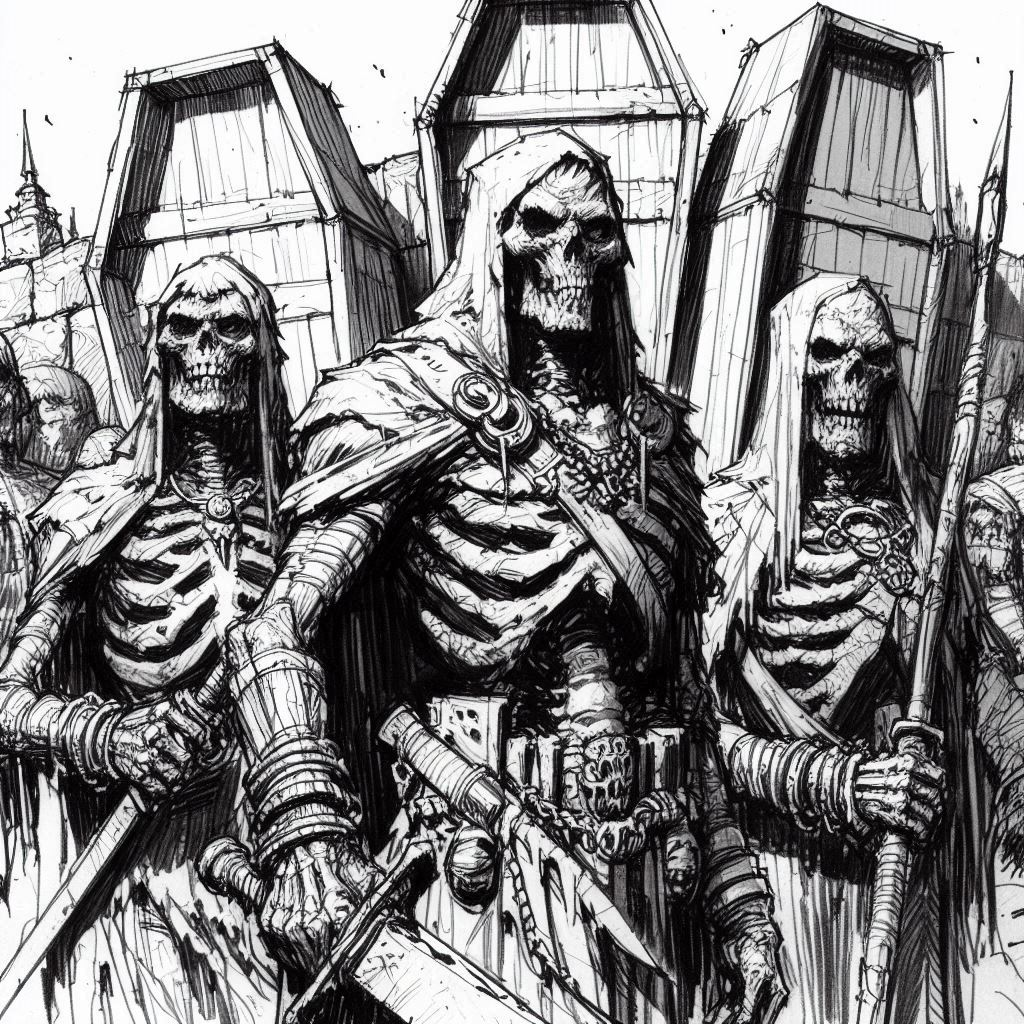
\includegraphics[width=\linewidth]{pics/squelette.jpg}
\end{center}
\vfill

\pagebreak
\section{Niveau 2}
\subsection{Fragments de Momie}\label{monster:s11}
\begin{itemize}
  \item \textbf{Apparence :}
  \begin{itemize}
    \item Bras noircis et décomposés
    \item Doigts acérés
  \end{itemize}
  \item \textbf{ Désirs :}  étrangler des choses, occire les vivants.
\end{itemize}

\SetTblrInner{hspan=minimal, vspan=even}
\begin{osrtable}{X[2]X[1]X[1]X[2]}{0}
  \SetCell[c=4]{bg=black,fg=white} {\bfseries\large\sectionfont Statistiques} & & &\\
  \textbf{CA}          & 7 [12] & \textbf{TACO}        & 19 [0] \\
  \textbf{Attaque}     & \SetCell[c=3]{l} 1D6 (griffes) & &\\
  \textbf{Sauvegardes} & \SetCell[c=3]{l} {\small \textbf{MP}~12 \textbf{B}~13 \textbf{PP}~14 \textbf{S}~15 \textbf{SSB}~16}& &\\
  \textbf{Mouvement} & 18m    & \textbf{Moral} & 12 \\
  \textbf{DV} & 1*   & \textbf{XP} & 13 \\
  \textbf{PV} (\hspace*{20pt}) & \SetCell[c=3]{l}\noindent\hdsquares{1} & &\\
  \textbf{PV} (\hspace*{20pt}) & \SetCell[c=3]{l}\noindent\hdsquares{1} & &\\
\end{osrtable}

\begin{itemize}
\item \textbf{Maladie :}
\begin{itemize}
  \item Maladie putrescente au toucher
  \item Guérison magique inefficace
  \item Guérison naturelle 10x plus longue
  \item Ne peut être éliminée que par magie
\end{itemize}
\item \textbf{Mort-vivant}
\begin{itemize}
  \item Silencieux.
  \item Insensible aux effets affectant les créatures vivantes.
  \item Immunisée contre les sorts affectant ou lisant l'esprit.
\end{itemize}
\end{itemize}

Ils se tortillent, grimpent votre corps et tentent de vous étrangler.

\vfill
%\pagebreak

\subsection{Sparamantur}\label{monster:s13}
\begin{itemize}
  \item \textbf{Apparence :}
  \begin{itemize}
    \item Squelette humain muni de crocs et d'une arme rouillée.
    \item Couvert de bracelets.
  \end{itemize}
  \item \textbf{ Désirs :} protéger le reste de la Tombe des Rois Serpents et tuer tout intrus.
\end{itemize}

\SetTblrInner{hspan=minimal, vspan=even}
\begin{osrtable}{X[2]X[1]X[1]X[2]}{0}
  \SetCell[c=4]{bg=black,fg=white} {\bfseries\large\sectionfont Statistiques} & & &\\
  \textbf{CA}          & 7 [12] & \textbf{TACO}        & 17 [2] \\
  \textbf{Attaque}     & \SetCell[c=3]{l} 1D8 (Hache de bataille) & &\\
  \textbf{Déplacement} & 18m    & \textbf{Moral} & 12 \\
  \textbf{Sauvegardes} & \SetCell[c=3]{l} {\small \textbf{MP}~12 \textbf{B}~13 \textbf{PP}~14 \textbf{S}~15 \textbf{SSB}~16}& &\\
  \textbf{Mouvement} & 18m    & \textbf{Moral} & 12 \\
  \textbf{DV} & 3   & \textbf{XP} & 35 \\
  \textbf{PV} (\hspace*{20pt}) & \SetCell[c=3]{l}\noindent\hdsquares{3} & &\\
\end{osrtable}

\begin{itemize}
  \item Ne subit que la moitié des dégâts infligés par les armes perçantes ou tranchantes.
  \item Il craque et cliquette, meurtrier et implacable
\end{itemize}

\vfill
%\pagebreak

\subsection{Pudding Noir (Franbinzar)}\label{monster:s14}
\begin{itemize}
  \item \textbf{Apparence :}  100 kg de mélasse noire
  \item \textbf{ Désirs :} Se nourrir.
\end{itemize}

\begin{osrtable}{X[2]X[1]X[1]X[2]}{0}
 \SetCell[c=4]{bg=black,fg=white} {\bfseries\large\sectionfont Statistiques} & & &\\
 \textbf{CA}          & 6 [13] & \textbf{TACO}        & 15 [4] \\
 \textbf{Attaque}     & \SetCell[c=3]{l} 2D8 (toucher) & &\\
 \textbf{Sauvegardes} & \SetCell[c=3]{l} {\small \textbf{MP}~10 \textbf{B}~11 \textbf{PP}~12 \textbf{S}~13 \textbf{SSB}~14}& &\\
 \textbf{Mouvement} & 18m    & \textbf{Moral} & 12 \\
 \textbf{DV} &  5   & \textbf{XP} & 300 \\
 \textbf{PV} (\hspace*{20pt}) & \SetCell[c=3]{l}\noindent\hdsquares{5} & &\\
\end{osrtable}

\begin{itemize}
  \item \textbf{Immunité :} Blessé uniquement par le feu, autres: dégâts temporaires
  \item \textbf{Division :} Les attaques qui ne sont pas liées au feu (y compris les sorts) provoquent la division du pudding. Chaque coup crée un nouveau pudding de 1 DV qui inflige 1d6 points de dégâts.
  \item \textbf{Corrosion :} Peut dissoudre le bois ou le métal en un tour (10\% de chances).
  \item \textbf{Collant :} Peut se déplacer sur les murs et les plafonds.
  \item \textbf{Suintement :} Peut s'infiltrer à travers les petits trous et fissures.
  \item \textbf{Régénération :} Si tué, se régénère en 1d20 heures, à moins d'être incinéré.
  \item \textbf{Attaques multiples :} Peut cibler tous les PJ adjacents à chaque round, effectuant un jet d'attaque classique pour chacun.
\end{itemize}

Franbinzar était le dernier roi de la forteresse.

Sa momification ne s'est pas déroulée correctement.
Il s'est transformé en Pudding Noir.

On peut apercevoir 200PO d'anneaux noyés dans sa masse.

\vfill

%\columnbreak

\subsection{Gardien Cobra de Pierre}\label{monster:s19}
\begin{itemize}
  \item \textbf{Apparence :}
  \begin{itemize}
    \item  Chevalier de pierre vêtu d'une armure sculptée.
    \item Une de ses mains manie une imposante épée dentelée.
    \item L'autre est libre au début du combat.
  \end{itemize}
  \item \textbf{ Désirs :}  protéger le reste de la Tombe des Rois Serpents et  tuer les intrus.
\end{itemize}

\begin{osrtable}{X[2]X[1]X[1]X[2]}{0}
  \SetCell[c=4]{bg=black,fg=white} {\bfseries\large\sectionfont Statistiques} & & &\\
  \textbf{CA}          & 3 [16] & \textbf{TACO}        & 15 [4] \\
  \textbf{Attaque}     & \SetCell[c=3]{l} 2D6 (épée dentelée) & &\\
  \textbf{Sauvegardes} & \SetCell[c=3]{l} {\small \textbf{MP}~10 \textbf{B}~11 \textbf{PP}~12 \textbf{S}~13 \textbf{SSB}~14}& &\\
  \textbf{Mouvement} & 18m    & \textbf{Moral} & 12 \\
  \textbf{DV} &  4+1   & \textbf{XP} & 125 \\
  \textbf{PV} (\hspace*{20pt}) & \SetCell[c=3]{l}\noindent\hdsquares{4}~$\square$ & &\\
\end{osrtable}

\textbf{Attaques :} Chaque round, le Gardien Cobra de Pierre peut
appliquer une de ces stratégies :
\begin{enumerate}
  \item \textbf{Appel du Bouclier :}
  Le Gardien appelle à lui un des boucliers couvrant les murs de l'arène.
  \begin{itemize}
    \item 1d6 dégâts (jet de sauvegarde contre la mort pour esquiver) si sur trajectoire
    \item Garde le bouclier (+1 CA)
  \end{itemize}
  \item \textbf{Bond et Impact :}
  Le Gardien bondit à travers les airs puis plonge jusqu'à 6 m de sa position initiale.
  \begin{itemize}
    \item toute créature adjacente : 1d4 dégâts (sauvegarde contre la mort annule).
    \item si dégât : projeté au sol
  \end{itemize}
  \item \textbf{Attaque normale}
\end{enumerate}

\textbf{Stratégies possibles :}
\begin{itemize}
  \item Prendre le Gardien en \textbf{tenaille}
  \item \textbf{Fuir :} Trop imposant pour l'escalier
  \item \textbf{Courir :} suit le PJ tant que détectables
\end{itemize}

\vfill
\pagebreak

\section{Niveau 3}
\subsection{Monstres Errants}\label{monster:n3:errants}
\begin{enumerate}
  \item \textbf{Présage du Basilic.}
  Des cliquetis et grincements d'une chaîne distante traînée sur de la roche et dans la poussière.
  \item \textbf{Présage de Gelées Squelettes.}
  Des bruits de succion résonnant dans le lointain.
  \item \textbf{Présage de Gobelins.}
  \begin{itemize}
    \item Chuchotis, gloussements, grincements de dents et pourléchage de babines.
    \item Le reflet d'yeux rouges dans l'obscurité.
    \item Un fumet de pourriture fongique.
  \end{itemize}
  \item \textbf{Chauve-souris.}
  Nullement hostile, mais effrayante sur le moment.
  Volette de-ci de-là, plane en direction du gouffre.
  \item \textbf{\nameref{monster:n3:araignee}}
  \item \textbf{1d6 \nameref{monster:n3:gob}} en reconnaissance.
  \begin{itemize}
    \item 1d6 autres gobelins fongiques postés au détour du prochain couloir.
  \end{itemize}
  \item  \textbf{1 \nameref{monster:n3:squelgel}.}
  \item  \textbf{1d10+5 \nameref{monster:n3:gob}} parés au combat.\\
  L'un d'eux est muni d'une lance faite de couverts, absurdement peu pratique à manier (1d6 dégâts, allonge)
\end{enumerate}


%\pagebreak
\subsection{Grosse Araignée}\label{monster:n3:araignee}
  \begin{itemize}
  \item De la taille d'un poing.
  \item Cherche à manger des chauves-souris, pas les PJ.
  \item \textbf{Venimeuse : } 1d4 dégâts
  \begin{itemize}
    \item sauvegarde poison annule
  \end{itemize}
  \item \textbf{lâche}
  \item Mets de choix pour les gobelins fongiques.
\end{itemize}

\SetTblrInner{hspan=minimal, vspan=even}
\begin{osrtable}{X[2]X[1]X[1]X[2]}{0}
  \SetCell[c=4]{bg=black,fg=white} {\bfseries\large\sectionfont Statistiques} & & &\\
  \textbf{CA}          & 7 [12] & \textbf{TACO}        & 19 [0] \\
  \textbf{Attaque}     & \SetCell[c=3]{l} 1D3 (morsure) + poison & &\\
  \textbf{Sauvegardes} & \SetCell[c=3]{l} {\small \textbf{MP}~12 \textbf{B}~13 \textbf{PP}~14 \textbf{S}~15 \textbf{SSB}~16}& &\\
  \textbf{Mouvement} & 9m    & \textbf{Moral} & 8 \\
  \textbf{DV} & 1/2   & \textbf{XP} & 5 \\
  \textbf{PV} (\hspace*{20pt}) & \SetCell[c=3]{l}\noindent$\square\square\square\square$ & &\\
\end{osrtable}


\vfill
%\columnbreak
\subsection{Gelée Squelette}\label{monster:n3:squelgel}
\begin{itemize}
  \item \textbf{Apparence :} Un squelette couvert de mucus orange
  \item \textbf{Désirs :}  écraser des crânes et créer plus de gelées squelettes.
\end{itemize}

\SetTblrInner{hspan=minimal, vspan=even}
\begin{osrtable}{X[2]X[1]X[1]X[2]}{0}
  \SetCell[c=4]{bg=black,fg=white} {\bfseries\large\sectionfont Statistiques} & & &\\
  \textbf{CA}          & 7 [12] & \textbf{TACO}        & 19 [0] \\
  \textbf{Attaque}     & \SetCell[c=3]{l} 1D4 (griffes) & &\\
  \textbf{Sauvegardes} & \SetCell[c=3]{l} {\small \textbf{MP}~12 \textbf{B}~13 \textbf{PP}~14 \textbf{S}~15 \textbf{SSB}~16}& &\\
  \textbf{Mouvement} & 9m    & \textbf{Moral} & 12 \\
  \textbf{DV} & 2   & \textbf{XP} & 20 \\
  \textbf{PV} (\hspace*{20pt}) & \SetCell[c=3]{l}N.A. & &\\
  \textbf{PV} (\hspace*{20pt}) & \SetCell[c=3]{l}N.A. & &\\
  \textbf{PV} (\hspace*{20pt}) & \SetCell[c=3]{l}N.A. & &\\
  \textbf{PV} (\hspace*{20pt}) & \SetCell[c=3]{l}N.A. & &\\
\end{osrtable}

\begin{itemize}
  \item Immunisés à tous dommages.
  \item \textbf{Solutions possibles:}
  \begin{itemize}
    \item Fuir,
    \item les faire pétrifier par le \textbf{\nameref{monster:n3:basilic}},
    \item les précipiter dans le gouffre,
    \item les attacher
    \item les enfermer dans une salle
    \item les précipiter en \textbf{\nameref{n3:s25}} ou \textbf{\nameref{n3:s37}}
  \end{itemize}
  \item Sortent des fosses / se libérent des cordes (temps variable).
  \item \textbf{4} gelées squelettes en tout
  \begin{itemize}
    \item Vaincue : retirer de la \textbf{Table des \nameref{monster:n3:errants}}
  \end{itemize}
  \item \textbf{Contagion:} Toute victime (tuée) devient une gelée squelette en 10 minutes.
  \begin{itemize}
    \item \textbf{\nameref{monster:n3:gob}} immunisés.
  \end{itemize}
\end{itemize}


\vfill

\subsection{Gobelins Fongiques}\label{monster:n3:gob}
\SetTblrInner{hspan=minimal, vspan=even}
\begin{osrtable}{X[2]X[1]X[1]X[2]}{0}
  \SetCell[c=4]{bg=black,fg=white} {\bfseries\large\sectionfont Statistiques} & & &\\
  \textbf{CA}          & 6 [13] & \textbf{TACO}        & 19 [0] \\
  \textbf{Attaque}     & \SetCell[c=3]{l} 1D6 (arme) & &\\
  \textbf{Sauvegardes} & \SetCell[c=3]{l} {\small \textbf{MP}~14 \textbf{B}~15 \textbf{PP}~16 \textbf{S}~17 \textbf{SSB}~18}& &\\
  \textbf{Mouvement} & 18m    & \textbf{Moral} & 7 \\
  \textbf{DV} & 1-1   & \textbf{XP} & 5 \\
  \textbf{PV} (\hspace*{20pt}) & \SetCell[c=3]{l}\noindent\hdsquares{1} & &\\
  \textbf{PV} (\hspace*{20pt}) & \SetCell[c=3]{l}\noindent\hdsquares{1} & &\\
  \textbf{PV} (\hspace*{20pt}) & \SetCell[c=3]{l}\noindent\hdsquares{1} & &\\
  \textbf{PV} (\hspace*{20pt}) & \SetCell[c=3]{l}\noindent\hdsquares{1} & &\\
  \textbf{PV} (\hspace*{20pt}) & \SetCell[c=3]{l}\noindent\hdsquares{1} & &\\
  \textbf{PV} (\hspace*{20pt}) & \SetCell[c=3]{l}\noindent\hdsquares{1} & &\\
  \textbf{PV} (\hspace*{20pt}) & \SetCell[c=3]{l}\noindent\hdsquares{1} & &\\
\end{osrtable}

\begin{itemize}
  \item \textbf{Apparence :}
  \begin{itemize}
    \item pâles et rabougris,
    \item \'Enorme tête ovale
    \item Plein de dents et deux petits yeux rouges beaucoup trop près l'un de l'autre.
    \item Texture évoque une purée de pommes de terre à la colle blanche.
    \item Portent sur eux des couverts de  table.
  \end{itemize}
  \item \textbf{ Désirs :} un roi, à manger, des choses qui brillent, encore à manger
  \item \textbf{Non hostiles :} ils cherchent seulement à couronner quelqu'un Roi des Gobelins (Initialement)
  \item \textbf{Dialecte :} gobelin cliquetant et limité.
  \item Aisément \textbf{corruptibles}
  \item Si PJ hostiles:
  \begin{itemize}
    \item \textbf{Fuite}
    \item \textbf{Embuscades} récurrentes
    \item Sournois et patients
    \item Escaladent (lentement) les murs : surprendre les aventuriers en leur plongeant dessus
    \item Seaux d'eau pour éteindre les torches
    \item Cordes pour emmêler les combattants
    \item Tirent profit des pièges du donjon
    \item De nuit, harcèlent le campement
  \end{itemize}
  \item \textbf{Roi des gobelins :} destin
  \begin{itemize}
    \item suivi jusqu'à la pleine lune
    \item puis assailli, traîné jusqu'à un autel au sommet d'une colline et éventré
  \end{itemize}
  \item \textbf{Connaissances :}
  \begin{itemize}
    \item Peuvent avertir au sujet du \textbf{\nameref{monster:n3:basilic}}
    \item Ignorent l'existence du \textbf{\nameref{n3:s39}}
    \item Ignorent tout des niveaux supérieurs : bloqués par le \textbf{\nameref{monster:s19}}
  \end{itemize}
\end{itemize}

La nuit venue, ils utilisent \textbf{\nameref{n3:s41}} pour se faufiler jusqu'à l'extérieur.

À moins que \textbf{\nameref{n3:s48}} ne soit incendiée, le nombre de gobelins dans le donjon sera toujours "beaucoup trop de gobelins".

Les gobelins fongiques sont des rats de laboratoire parvenus à s'échapper.
Bien que \textbf{\nameref{monster:n3:xiximanter}} ne s'oppose pas à ce qu'on les lui rende, ils ne lui sont pas d'une grande utilité.

\vfill
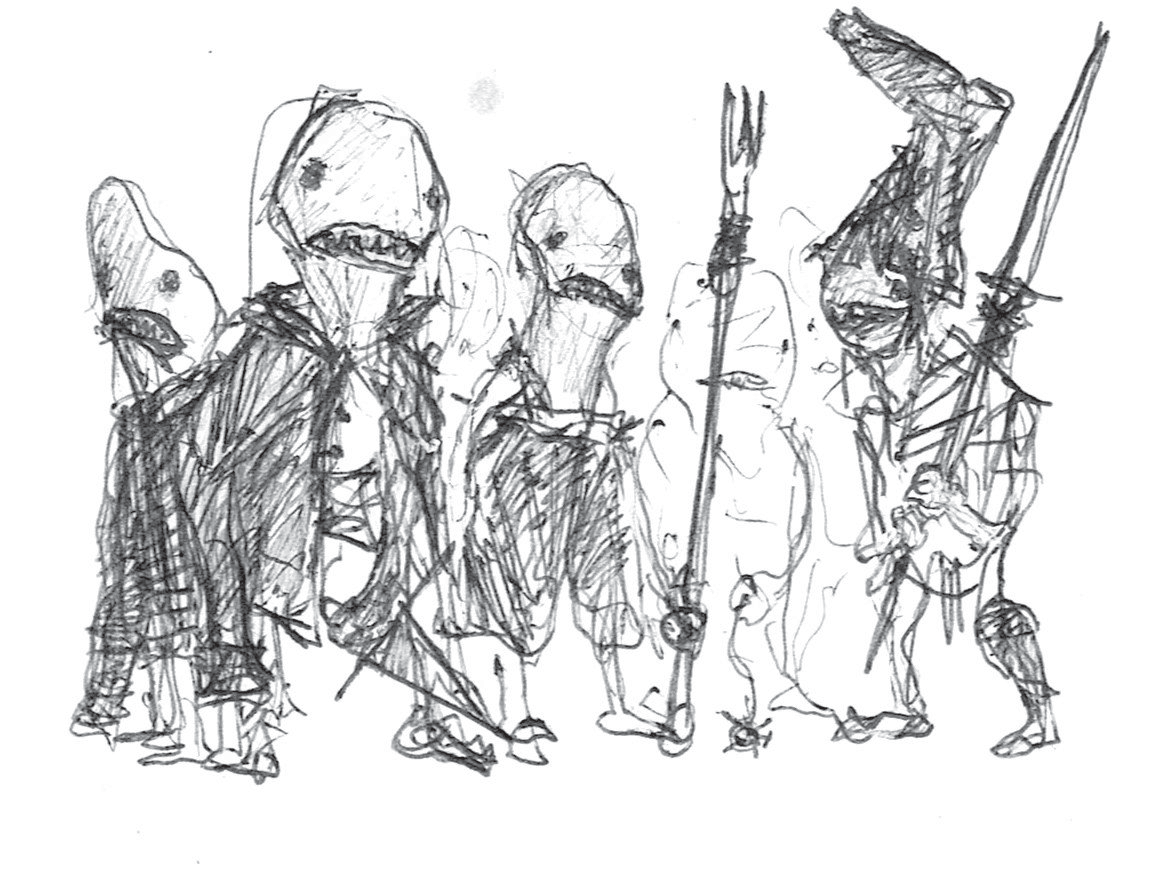
\includegraphics[width=\columnwidth]{pics/gob.png}

\pagebreak
\subsection{Succube}\label{monster:n3:succube}
\begin{itemize}
  \item \textbf{Apparence :}  Jeune botaniste de la race du premier PJ qu'il aperçoit, et de sexe approprié
  \item \textbf{ Désirs :}
  \begin{itemize}
    \item \textbf{Recharger ses réserves :} embrasser un PJ (drain)
    \item \textbf{S'échapper :} pousser quelqu'un à s'approcher et franchir le cercle de confinement.
  \end{itemize}
\end{itemize}

\SetTblrInner{hspan=minimal, vspan=even}
\begin{osrtable}{X[2]X[1]X[1]X[2]}{0}
  \SetCell[c=4]{bg=black,fg=white} {\bfseries\large\sectionfont Statistiques} & & &\\
  \textbf{CA}          & 2 [17] & \textbf{TACO}        & 14 [+5] \\
  \textbf{Attaque}     & \SetCell[c=3]{l} 1D3 (2 $\times$ griffes) & &\\
  \textbf{Sauvegardes} & \SetCell[c=3]{l} {\small \textbf{MP}~10 \textbf{B}~11 \textbf{PP}~12 \textbf{S}~13 \textbf{SSB}~14}& &\\
  \textbf{Mouvement} & 18m    & \textbf{Moral} & 10 \\
  \textbf{DV} & 6*  & \textbf{XP} & 500 \\
  \textbf{PV} (\hspace*{20pt}) & \SetCell[c=3]{l}\noindent\hdsquares{6} & &\\
\end{osrtable}

\begin{itemize}
  \item \textbf{Immunité :} Pétrification, Feu et armes non magiques
  \item \textbf{Drain d'énergie :} Un baiser draine d'un niveau. Sauvegarde contre la mort annule
  \item \textbf{Sorts :} Charme-personne, Image miroir
  \item Son nom véritable (\textbf{Baltoplate}) figure  sur un parchemin en salle \textbf{\nameref{n2:s15}}
  \item Fuit tout combat, refuse de s'y risquer.
  \item Ne revient pas ensuite.
  \item Si doit marchander pour sa vie / liberté, , il peut proposer de :
  \begin{itemize}
    \item Détecter les poisons,
    \item Révéler d'anciens secrets
    \item Tuer n'importe quelle personne mortelle que les PJ peuvent nommer
  \end{itemize}
  \item Patient et fourbe, mais tient toujours parole
\end{itemize}

\vfill\
\begin{center}
  \vspace*{0.2\textheight}
  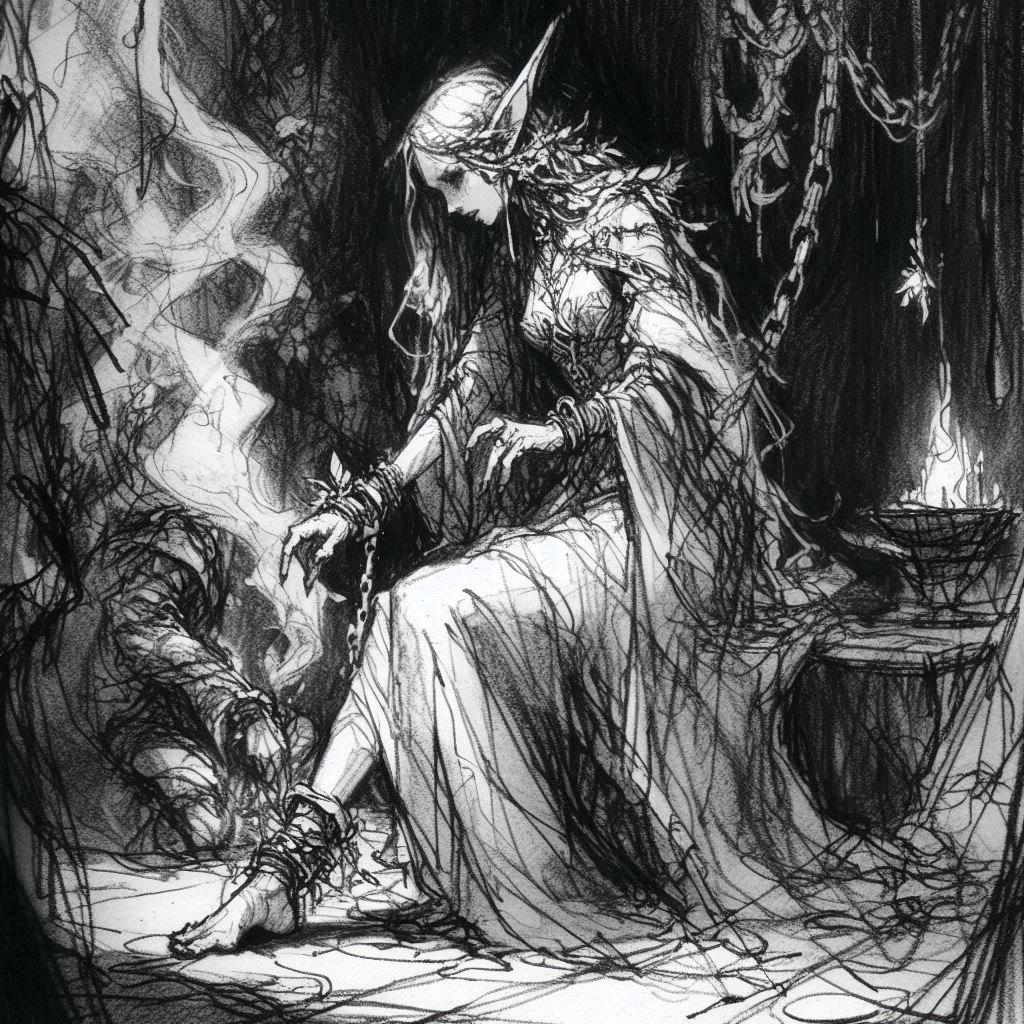
\includegraphics[width=\linewidth]{pics/succube.jpg}
\end{center}
\vfill

\pagebreak
\subsection{Basilic}\label{monster:n3:basilic}
\begin{itemize}
  \item \textbf{Apparence :}
  \begin{itemize}
    \item titanesque lézard octopède à tête crocodilienne aplatie et pleine de dents.
    \item \OE illères de bronze vissées dans le crâne
    \item Collier autour du cou, juste devant sa première paire de pattes.
  \end{itemize}
  \item \textbf{ Désirs :} nourriture, chaleur et liberté.
\end{itemize}

\SetTblrInner{hspan=minimal, vspan=even}
\begin{osrtable}{X[2]X[1]X[1]X[2]}{0}
  \SetCell[c=4]{bg=black,fg=white} {\bfseries\large\sectionfont Statistiques} & & &\\
  \textbf{CA}          & 4 [15] & \textbf{TACO}        & 13 [+6]  \\
  \textbf{Attaque}     & \SetCell[c=3]{l} 1 morsure (1d10 + pétrification) & &\\
  \textbf{Attaque}     & \SetCell[c=3]{l} 1 regard (pétrification)  & &\\
  \textbf{Attaque}     & \SetCell[c=3]{l} 1 coup de queue (1D8 + projection)  & &\\
  \textbf{Sauvegardes} & \SetCell[c=3]{l} {\small \textbf{MP}~10 \textbf{B}~11 \textbf{PP}~12 \textbf{S}~13 \textbf{SSB}~14}& &\\
  \textbf{Mouvement} & 18m    & \textbf{Moral} & 10 \\
  \textbf{DV} & 6+1*  & \textbf{XP} & 950 \\
  \textbf{PV} (\hspace*{20pt}) & \SetCell[c=3]{l}\noindent\hdsquares{6}~$\square$ & &\\
\end{osrtable}

\begin{itemize}
  \item \textbf{Surprise :} Les personnages surpris par le basilic subissent une attaque de son regard pétrifiant.
  \item \textbf{Éviter son regard :} Une personne qui cherche à combattre le basilic en évitant son regard subit un malus de –4 pour toucher, tandis que le basilic bénéficie d'un bonus de +2.
  \item \textbf{Utiliser un miroir :} Le reflet du basilic est inoffensif. Se battre en regardant dans un miroir inflige un malus de –1 à l'attaque. Si le basilic voit son propre reflet (2 chances sur 6), il doit effectuer un jet de sauvegarde ou être pétrifié.
  \item \textbf{Pétrification :}
  \begin{itemize}
    \item \textbf{Simple coup d'\oe il:} légère sensation de pression
    \item \textbf{Fixe 1 round :} les membres sont lents, pesants, les pensées ralentissent.
    Immobile et -4 à la défense (sauvegarde contre la Pétrification annule).
    L'effet prend fin dès que le basilic détourne le regard.
    \item \textbf{Fixe 2 rounds :} Transformé en pierre (sauvegarde contre la Pétrification annule).
    Si réussite, reste cependant fixée sur place.
  \end{itemize}
  \item \OE illères peuvent être fermées
  \item \textbf{Comportement :}
  \begin{itemize}
    \item \textbf{Affamé (par défaut) :} se mouvant lentement dans l'obscurité, humant l'air, cherchant à identifier une proie isolée.
    Il se tient sur ses gardes si le groupe déclenche le piège du \textbf{\nameref{n3:s35}} ou ouvre la porte du \textbf{\nameref{n3:s39}}.
    \item \textbf{En digestion (si repus) :} lové dans un coin, dos au  mur, la tête relevée et paré à réagir.
    3 chances sur 6 d'être endormi.
    \item \textbf{Curieux (si repus) :} humant l'air, dodelinant de la tête pour éviter de pétrifier quelque chose par accident.
    Il peut reconnaître ceux qui l'ont nourri à l'odeur (lézard apprivoisé, il a appris  à ne pas mordre la main qui le nourrit).
    \item \textbf{Rage (si effrayé ou blessé) :} bondit en arrière de 3 m, dresse la queue et charge une cible dans le même tour.
    Celle-ci doit effectuer un jet de sauvegarde contre la paralysie .
  \end{itemize}
  \item Repus avec :
  \begin{itemize}
    \item 30 rations de voyage
    \item 2 humains normaux
    \item 1 cheval
    \item 6 gobelins fongiques
  \end{itemize}
\end{itemize}

Les mages et alchimistes accordent une grande valeur aux yeux du basilic (300 PO chaque).

Ses glandes salivaires contiennent l'équivalent de 2 potions de "Transmutation de la Pierre en Chair".

Son squelette pierreux peut se revendre 1000 PO, ou 300 PO pour la tête seule.

Vivante, la bête peut s'échanger contre 10.000 PO dans une ménagerie, le double si elle est domestiquée.

\vfill
\pagebreak
\subsection{Xiximanter}\label{monster:n3:xiximanter}
\begin{itemize}
  \item \textbf{Apparence :}
  \begin{itemize}
    \item Buste humain desséché
    \item Queue de serpent squelettique.
    \item Haillons d'une robe de mage
    \item Charmes et amulettes pendent à son cou.
    \item Deux yeux rouges, brûlant telles des aiguilles de feu.
    \item Deux crocs acérés.
    \item Toujours poli.
  \end{itemize}
  \item \textbf{ Désirs :}  êtres vivants, sorts, ingrédients rares pour potions
\end{itemize}

\SetTblrInner{hspan=minimal, vspan=even}
\begin{osrtable}{X[2]X[1]X[1]X[2]}{0}
  \SetCell[c=4]{bg=black,fg=white} {\bfseries\large\sectionfont Statistiques} & & &\\
  \textbf{CA}          & 1 [18] & \textbf{TACO}        & 11 [+8]  \\
  \textbf{Attaque}     & \SetCell[c=3]{l} 1 griffes (1d8 + paralysie) & &\\
  \textbf{Sauvegardes} & \SetCell[c=3]{l} {\small \textbf{MP}~6 \textbf{B}~7 \textbf{PP}~8 \textbf{S}~9 \textbf{SSB}~10}& &\\
  \textbf{Mouvement} & 18m    & \textbf{Moral} & 10 \\
  \textbf{DV} & 10***  & \textbf{XP} & 3700 \\
  \textbf{PV} (\hspace*{20pt}) & \SetCell[c=3]{l}\noindent\hdsquares{10} & &\\
\end{osrtable}

\begin{itemize}
  \item \textbf{Mort-vivant :} Silencieux jusqu'à l'attaque.
  Immunisé contre les effets qui affectent les créatures vivantes (par exemple le poison).
  Immunisé contre les sorts affectant l'esprit (par exemple, charme, immobilisation, sommeil).
  \item \textbf{Immunité :} Armes non magiques, électricité, froid, tous les sorts qui provoquent la métamorphose, la folie, la mort.
  \item \textbf{Aura de peur :} Xiximanter peut décider d'activer/désactiver son aura de peur.
  Ceux qui le voient doivent effectuer un jet de sauvegarde contre les sorts ou fuir pendant 2d6 tours.
  Les personnages de niveau 4 ou plus sont immunisés.
  \item \textbf{Griffe paralysante :} sauvegarde contre la paralysie ou paralysé pendant 6 tours.
  \item \textbf{Sorts mémorisés:} Comme un mage de niveau 10.
  \begin{itemize}
    \item \textbf{Niveau 1 :} Projectile magique, Sommeil, Charme-personne
    \item \textbf{Niveau 2 :} Invisibilité, ESP, Détection de l'invisible
    \item \textbf{Niveau 3 :} Boule de feu, Foudre, Paralysie
    \item \textbf{Niveau 4 :} Mur de feu, Confusion, Allométamorphose
    \item \textbf{Niveau 5 :} Débilité mentale, Téléportation
  \end{itemize}
  \item \textbf{Attitude :}
  \begin{itemize}
    \item Raisonnable, avenant (\emph{"Bonjour, bipèdes"})
    \item Besoin de créatures vivantes, de préférence intelligentes, des sorciers dans l'idéal.
    \item Les distille pour élaborer ses potions
    \item Croit fermement être sur le point de faire une découverte révolutionnaire
    \item Croit que la ville des hommes-serpents s'étend toujours à la surface, que la tombe est pleine de prêtres
    \item Entre dans une rage folle si confronté à la réalité
  \end{itemize}
\end{itemize}

\end{document}